\documentclass[11pt,a4paper]{article}
\usepackage[margin=2.3cm]{geometry}
\usepackage{amsmath,amssymb,bm}
\usepackage{graphicx}
\usepackage{booktabs}
\usepackage{upgreek}
\usepackage[dvipsnames]{xcolor}
\newenvironment{updenv}{\color{OliveGreen}}{}
\newcommand{\upd}[1]{{\color{OliveGreen}#1}}
\usepackage[colorlinks=true,linkcolor=NavyBlue,citecolor=NavyBlue,urlcolor=NavyBlue]{hyperref}
\usepackage[capitalise,noabbrev]{cleveref}

% notation of manuscript/manuscript.tex
\newcommand{\Q}{\mathbf{Q}}
\renewcommand{\H}{\mathbf{H}}
\newcommand{\J}{\mathbf{J}}
\newcommand{\U}{\mathbf{U}}
\renewcommand{\u}{\bm{u}}
\renewcommand{\r}{\mathbf{r}}
\newcommand{\nh}{\hat{\bm{n}}}
\newcommand{\la}{\left\langle}
\newcommand{\ra}{\right\rangle}
\newcommand{\ab}{{\alpha\beta}}
\newcommand{\mn}{{\mu\nu}}
\newcommand{\xir}{\xi_\mathrm{r}}
\newcommand{\elld}{\ell_\mathrm{d}}
\newcommand{\ii}{\mathrm{i}}
\newcommand{\ee}{\mathrm{e}}
\newcommand{\micron}{\upmu\mathrm{m}}
\newcommand{\minute}{\mathrm{min}}
\newcommand{\dbar}{\bar\partial}
\newcommand{\pd}[2]{\frac{\partial #1}{\partial #2}}

\title{The comoving $+1/2$ defect in the full model:\\
exact closure, the $\nabla\H$ terms and the density fluctuations}
\author{Report, \texttt{report\_full\_solution/}}
\date{12 October 2026; fluctuations added 17 October 2026; reduced model 23 October 2026}

% numbers quoted in the text, generated from the runs by collect_numbers.py
% generated by collect_numbers.py -- do not edit
\newcommand{\numSInfUniform}{0.846}
\newcommand{\numSwallFull}{0.844}
\newcommand{\numSwallMxFull}{0.845}
\newcommand{\numSwallMxPaper}{0.898}
\newcommand{\numSwallMxPlusR}{0.845}
\newcommand{\numSwallMxPlusT}{0.900}
\newcommand{\numSwallPaper}{0.898}
\newcommand{\numSwallPlusR}{0.844}
\newcommand{\numSwallPlusT}{0.898}
\newcommand{\numSwallPxFull}{0.841}
\newcommand{\numSwallPxPaper}{0.899}
\newcommand{\numSwallPxPlusR}{0.841}
\newcommand{\numSwallPxPlusT}{0.894}
\newcommand{\numampCoeffFull}{-0.18}
\newcommand{\numampCoeffLow}{0.81}
\newcommand{\numdevFullRZeropFive}{2.1}
\newcommand{\numdevFullROnepZero}{4.1}
\newcommand{\numdevFullRTwopZero}{7.7}
\newcommand{\numdevFullRFivepZero}{13.2}
\newcommand{\numdevPaperRZeropFive}{0.2}
\newcommand{\numdevPaperROnepZero}{0.3}
\newcommand{\numdevPaperRTwopZero}{0.9}
\newcommand{\numdevPaperRFivepZero}{3.4}
\newcommand{\numdevPlusRRZeropFive}{2.4}
\newcommand{\numdevPlusRROnepZero}{4.4}
\newcommand{\numdevPlusRRTwopZero}{7.6}
\newcommand{\numdevPlusRRFivepZero}{12.0}
\newcommand{\numdevPlusTRZeropFive}{2.6}
\newcommand{\numdevPlusTROnepZero}{4.9}
\newcommand{\numdevPlusTRTwopZero}{8.7}
\newcommand{\numdevPlusTRFivepZero}{13.9}
\newcommand{\numfActiveMaxFull}{14.8}
\newcommand{\numfActiveMaxPaper}{13.1}
\newcommand{\numfActiveMaxPlusR}{12.3}
\newcommand{\numfActiveMaxPlusT}{13.4}
\newcommand{\numfElasticMaxFull}{2.3}
\newcommand{\numfNetCoreFull}{-7.1}
\newcommand{\numfNetCorePaper}{-7.1}
\newcommand{\numfNetCorePlusR}{-7.0}
\newcommand{\numfNetCorePlusT}{-7.6}
\newcommand{\numhminAOne}{0.075}
\newcommand{\numhminAOneHalf}{0.051}
\newcommand{\numhminBOne}{0.075}
\newcommand{\numhminCOne}{0.075}
\newcommand{\numhminFOneHalf}{0.051}
\newcommand{\numhminFTwo}{0.038}
\newcommand{\numhminGTwo}{0.038}
\newcommand{\numhminHOne}{0.075}
\newcommand{\numhminLFifteen}{0.076}
\newcommand{\numhminLForty}{0.075}
\newcommand{\numhminLTen}{0.075}
\newcommand{\numhminLThirty}{0.075}
\newcommand{\numhminZOne}{0.075}
\newcommand{\numhminZOneHalf}{0.051}
\newcommand{\numjacWorst}{3\times10^{-8}}
\newcommand{\numkUnstable}{1.8}
\newcommand{\numlfAOneFull}{3\times10^{-13}}
\newcommand{\numlfAOneHalfFull}{2\times10^{-11}}
\newcommand{\numlfAOneHalfPZero}{4\times10^{-13}}
\newcommand{\numlfAOneHalfPOne}{10^{-12}}
\newcommand{\numlfAOneHalfPTwo}{4\times10^{-13}}
\newcommand{\numlfAOnePZero}{7\times10^{-14}}
\newcommand{\numlfAOnePOne}{2\times10^{-13}}
\newcommand{\numlfAOnePTwo}{10^{-13}}
\newcommand{\numlfBOneBwR}{10^{-13}}
\newcommand{\numlfBOneBwRH}{10^{-13}}
\newcommand{\numlfBOneFull}{8\times10^{-13}}
\newcommand{\numlfBOnePZero}{7\times10^{-14}}
\newcommand{\numlfCOneFull}{4\times10^{-13}}
\newcommand{\numlfFOneHalfFull}{7\times10^{-13}}
\newcommand{\numlfFTwoFull}{10^{-12}}
\newcommand{\numlfGTwoPZero}{3\times10^{-13}}
\newcommand{\numlfHOneHlow}{3\times10^{-11}}
\newcommand{\numlfHOnePTwo}{9\times10^{-14}}
\newcommand{\numlfLFifteenFull}{2\times10^{-13}}
\newcommand{\numlfLFifteenPZero}{10^{-13}}
\newcommand{\numlfLFifteenPOne}{4\times10^{-13}}
\newcommand{\numlfLFifteenPTwo}{3\times10^{-13}}
\newcommand{\numlfLFortyFull}{2\times10^{-13}}
\newcommand{\numlfLFortyPZero}{6\times10^{-14}}
\newcommand{\numlfLFortyPOne}{2\times10^{-13}}
\newcommand{\numlfLFortyPTwo}{9\times10^{-14}}
\newcommand{\numlfLTenFull}{3\times10^{-12}}
\newcommand{\numlfLTenPZero}{5\times10^{-13}}
\newcommand{\numlfLTenPOne}{10^{-12}}
\newcommand{\numlfLTenPTwo}{10^{-12}}
\newcommand{\numlfLThirtyFull}{3\times10^{-13}}
\newcommand{\numlfLThirtyPZero}{10^{-13}}
\newcommand{\numlfLThirtyPOne}{3\times10^{-13}}
\newcommand{\numlfLThirtyPTwo}{10^{-13}}
\newcommand{\numlfZOneFull}{10^{-13}}
\newcommand{\numlfZOneHalfFull}{10^{-13}}
\newcommand{\numnxAOne}{101}
\newcommand{\numnxAOneHalf}{149}
\newcommand{\numnxBOne}{101}
\newcommand{\numnxCOne}{101}
\newcommand{\numnxFOneHalf}{149}
\newcommand{\numnxFTwo}{199}
\newcommand{\numnxGTwo}{199}
\newcommand{\numnxHOne}{101}
\newcommand{\numnxLFifteen}{95}
\newcommand{\numnxLForty}{121}
\newcommand{\numnxLTen}{91}
\newcommand{\numnxLThirty}{111}
\newcommand{\numnxZOne}{101}
\newcommand{\numnxZOneHalf}{149}
\newcommand{\numokAOneFull}{1}
\newcommand{\numokAOneHalfFull}{0}
\newcommand{\numokAOneHalfPZero}{1}
\newcommand{\numokAOneHalfPOne}{1}
\newcommand{\numokAOneHalfPTwo}{1}
\newcommand{\numokAOnePZero}{1}
\newcommand{\numokAOnePOne}{1}
\newcommand{\numokAOnePTwo}{1}
\newcommand{\numokBOneBwR}{1}
\newcommand{\numokBOneBwRH}{1}
\newcommand{\numokBOneFull}{1}
\newcommand{\numokBOnePZero}{1}
\newcommand{\numokCOneFull}{1}
\newcommand{\numokFOneHalfFull}{1}
\newcommand{\numokFTwoFull}{1}
\newcommand{\numokGTwoPZero}{1}
\newcommand{\numokHOneHlow}{0}
\newcommand{\numokHOnePTwo}{1}
\newcommand{\numokLFifteenFull}{1}
\newcommand{\numokLFifteenPZero}{1}
\newcommand{\numokLFifteenPOne}{1}
\newcommand{\numokLFifteenPTwo}{1}
\newcommand{\numokLFortyFull}{1}
\newcommand{\numokLFortyPZero}{1}
\newcommand{\numokLFortyPOne}{1}
\newcommand{\numokLFortyPTwo}{1}
\newcommand{\numokLTenFull}{1}
\newcommand{\numokLTenPZero}{1}
\newcommand{\numokLTenPOne}{1}
\newcommand{\numokLTenPTwo}{1}
\newcommand{\numokLThirtyFull}{1}
\newcommand{\numokLThirtyPZero}{1}
\newcommand{\numokLThirtyPOne}{1}
\newcommand{\numokLThirtyPTwo}{1}
\newcommand{\numokZOneFull}{1}
\newcommand{\numokZOneHalfFull}{1}
\newcommand{\numresAOneFull}{3\times10^{-12}}
\newcommand{\numresAOneHalfFull}{2\times10^{0}}
\newcommand{\numresAOneHalfPZero}{6\times10^{-12}}
\newcommand{\numresAOneHalfPOne}{3\times10^{-11}}
\newcommand{\numresAOneHalfPTwo}{5\times10^{-12}}
\newcommand{\numresAOnePZero}{3\times10^{-12}}
\newcommand{\numresAOnePOne}{3\times10^{-12}}
\newcommand{\numresAOnePTwo}{3\times10^{-11}}
\newcommand{\numresBOneBwR}{2\times10^{-12}}
\newcommand{\numresBOneBwRH}{3\times10^{-12}}
\newcommand{\numresBOneFull}{3\times10^{-12}}
\newcommand{\numresBOnePZero}{3\times10^{-12}}
\newcommand{\numresCOneFull}{3\times10^{-12}}
\newcommand{\numresFOneHalfFull}{4\times10^{-10}}
\newcommand{\numresFTwoFull}{9\times10^{-11}}
\newcommand{\numresGTwoPZero}{10^{-11}}
\newcommand{\numresHOneHlow}{7\times10^{-1}}
\newcommand{\numresHOnePTwo}{3\times10^{-12}}
\newcommand{\numresLFifteenFull}{3\times10^{-12}}
\newcommand{\numresLFifteenPZero}{3\times10^{-12}}
\newcommand{\numresLFifteenPOne}{4\times10^{-12}}
\newcommand{\numresLFifteenPTwo}{6\times10^{-11}}
\newcommand{\numresLFortyFull}{2\times10^{-12}}
\newcommand{\numresLFortyPZero}{2\times10^{-12}}
\newcommand{\numresLFortyPOne}{3\times10^{-12}}
\newcommand{\numresLFortyPTwo}{2\times10^{-12}}
\newcommand{\numresLTenFull}{2\times10^{-12}}
\newcommand{\numresLTenPZero}{3\times10^{-12}}
\newcommand{\numresLTenPOne}{3\times10^{-12}}
\newcommand{\numresLTenPTwo}{3\times10^{-12}}
\newcommand{\numresLThirtyFull}{2\times10^{-12}}
\newcommand{\numresLThirtyPZero}{2\times10^{-12}}
\newcommand{\numresLThirtyPOne}{2\times10^{-11}}
\newcommand{\numresLThirtyPTwo}{2\times10^{-12}}
\newcommand{\numresZOneFull}{3\times10^{-11}}
\newcommand{\numresZOneHalfFull}{10^{-11}}
\newcommand{\numrhalfHeadFull}{0.84}
\newcommand{\numrhalfHeadPaper}{1.03}
\newcommand{\numrhalfHeadPlusR}{1.02}
\newcommand{\numrhalfHeadPlusT}{0.99}
\newcommand{\numrhalfPade}{0.94}
\newcommand{\numrhalfSideFull}{0.80}
\newcommand{\numrhalfSidePaper}{0.96}
\newcommand{\numrhalfSidePlusR}{0.95}
\newcommand{\numrhalfSidePlusT}{0.92}
\newcommand{\numrhalfTailFull}{0.80}
\newcommand{\numrhalfTailPaper}{0.89}
\newcommand{\numrhalfTailPlusR}{0.95}
\newcommand{\numrhalfTailPlusT}{0.93}
\newcommand{\numrhoMaxFull}{1.88}
\newcommand{\numrhoMaxPaper}{0.20}
\newcommand{\numrhoMaxPlusR}{1.56}
\newcommand{\numrhoMaxPlusT}{1.79}
\newcommand{\numrhoMinFull}{-0.10}
\newcommand{\numrhoMinPaper}{-1.21}
\newcommand{\numrhoMinPlusR}{-0.10}
\newcommand{\numrhoMinPlusT}{-0.11}
\newcommand{\numtimeAOne}{16}
\newcommand{\numtimeAOneHalf}{27}
\newcommand{\numtimeBOne}{20}
\newcommand{\numtimeCOne}{7}
\newcommand{\numtimeFOneHalf}{2}
\newcommand{\numtimeFTwo}{4}
\newcommand{\numtimeGTwo}{1}
\newcommand{\numtimeHOne}{18}
\newcommand{\numtimeLFifteen}{17}
\newcommand{\numtimeLForty}{54}
\newcommand{\numtimeLTen}{14}
\newcommand{\numtimeLThirty}{19}
\newcommand{\numtimeZOne}{1}
\newcommand{\numtimeZOneHalf}{2}
\newcommand{\numuAOneFull}{-0.2264}
\newcommand{\numuAOneHalfFull}{-0.1970}
\newcommand{\numuAOneHalfPZero}{+0.2385}
\newcommand{\numuAOneHalfPOne}{-0.1378}
\newcommand{\numuAOneHalfPTwo}{-0.1964}
\newcommand{\numuAOnePZero}{+0.2385}
\newcommand{\numuAOnePOne}{-0.1379}
\newcommand{\numuAOnePTwo}{-0.1964}
\newcommand{\numuBOneBwR}{+0.2047}
\newcommand{\numuBOneBwRH}{+0.1735}
\newcommand{\numuBOneFull}{-0.2264}
\newcommand{\numuBOnePZero}{+0.2385}
\newcommand{\numuCOneFull}{-0.2264}
\newcommand{\numuErrOne}{6.8\times10^{-5}}
\newcommand{\numuErrOneRel}{0.03}
\newcommand{\numuExtrap}{-0.22637}
\newcommand{\numuFOneHalfFull}{-0.2264}
\newcommand{\numuFTwoFull}{-0.2264}
\newcommand{\numuFineAOneFull}{-0.2264418}
\newcommand{\numuFineAOneHalfFull}{-0.1970495}
\newcommand{\numuFineAOneHalfPZero}{+0.2385002}
\newcommand{\numuFineAOneHalfPOne}{-0.1378214}
\newcommand{\numuFineAOneHalfPTwo}{-0.1963723}
\newcommand{\numuFineAOnePZero}{+0.2384998}
\newcommand{\numuFineAOnePOne}{-0.1378980}
\newcommand{\numuFineAOnePTwo}{-0.1964310}
\newcommand{\numuFineBOneBwR}{+0.2047182}
\newcommand{\numuFineBOneBwRH}{+0.1734886}
\newcommand{\numuFineBOneFull}{-0.2264418}
\newcommand{\numuFineBOnePZero}{+0.2384998}
\newcommand{\numuFineCOneFull}{-0.2264418}
\newcommand{\numuFineFOneHalfFull}{-0.2263914}
\newcommand{\numuFineFTwoFull}{-0.2263796}
\newcommand{\numuFineGTwoPZero}{+0.2384998}
\newcommand{\numuFineHOneHlow}{-0.2217893}
\newcommand{\numuFineHOnePTwo}{-0.1964310}
\newcommand{\numuFineLFifteenFull}{-0.2627325}
\newcommand{\numuFineLFifteenPZero}{+0.2415648}
\newcommand{\numuFineLFifteenPOne}{-0.1667384}
\newcommand{\numuFineLFifteenPTwo}{-0.2301059}
\newcommand{\numuFineLFortyFull}{-0.1723725}
\newcommand{\numuFineLFortyPZero}{+0.2055139}
\newcommand{\numuFineLFortyPOne}{-0.0940807}
\newcommand{\numuFineLFortyPTwo}{-0.1444673}
\newcommand{\numuFineLTenFull}{-0.3348834}
\newcommand{\numuFineLTenPZero}{+0.2275177}
\newcommand{\numuFineLTenPOne}{-0.2243556}
\newcommand{\numuFineLTenPTwo}{-0.2957584}
\newcommand{\numuFineLThirtyFull}{-0.1901045}
\newcommand{\numuFineLThirtyPZero}{+0.2221982}
\newcommand{\numuFineLThirtyPOne}{-0.1088937}
\newcommand{\numuFineLThirtyPTwo}{-0.1619876}
\newcommand{\numuFineZOneFull}{+0.0000222}
\newcommand{\numuFineZOneHalfFull}{+0.0000039}
\newcommand{\numuGTwoPZero}{+0.2385}
\newcommand{\numuHOneHlow}{-0.2218}
\newcommand{\numuHOnePTwo}{-0.1964}
\newcommand{\numuLFifteenFull}{-0.2627}
\newcommand{\numuLFifteenPZero}{+0.2416}
\newcommand{\numuLFifteenPOne}{-0.1667}
\newcommand{\numuLFifteenPTwo}{-0.2301}
\newcommand{\numuLFortyFull}{-0.1724}
\newcommand{\numuLFortyPZero}{+0.2055}
\newcommand{\numuLFortyPOne}{-0.0941}
\newcommand{\numuLFortyPTwo}{-0.1445}
\newcommand{\numuLTenFull}{-0.3349}
\newcommand{\numuLTenPZero}{+0.2275}
\newcommand{\numuLTenPOne}{-0.2244}
\newcommand{\numuLTenPTwo}{-0.2958}
\newcommand{\numuLThirtyFull}{-0.1901}
\newcommand{\numuLThirtyPZero}{+0.2222}
\newcommand{\numuLThirtyPOne}{-0.1089}
\newcommand{\numuLThirtyPTwo}{-0.1620}
\newcommand{\numuLowAtMax}{-0.2218}
\newcommand{\numuSciAOneFull}{-2.3\times10^{-1}}
\newcommand{\numuSciAOneHalfFull}{-2.0\times10^{-1}}
\newcommand{\numuSciAOneHalfPZero}{2.4\times10^{-1}}
\newcommand{\numuSciAOneHalfPOne}{-1.4\times10^{-1}}
\newcommand{\numuSciAOneHalfPTwo}{-2.0\times10^{-1}}
\newcommand{\numuSciAOnePZero}{2.4\times10^{-1}}
\newcommand{\numuSciAOnePOne}{-1.4\times10^{-1}}
\newcommand{\numuSciAOnePTwo}{-2.0\times10^{-1}}
\newcommand{\numuSciBOneBwR}{2.0\times10^{-1}}
\newcommand{\numuSciBOneBwRH}{1.7\times10^{-1}}
\newcommand{\numuSciBOneFull}{-2.3\times10^{-1}}
\newcommand{\numuSciBOnePZero}{2.4\times10^{-1}}
\newcommand{\numuSciCOneFull}{-2.3\times10^{-1}}
\newcommand{\numuSciFOneHalfFull}{-2.3\times10^{-1}}
\newcommand{\numuSciFTwoFull}{-2.3\times10^{-1}}
\newcommand{\numuSciGTwoPZero}{2.4\times10^{-1}}
\newcommand{\numuSciHOneHlow}{-2.2\times10^{-1}}
\newcommand{\numuSciHOnePTwo}{-2.0\times10^{-1}}
\newcommand{\numuSciLFifteenFull}{-2.6\times10^{-1}}
\newcommand{\numuSciLFifteenPZero}{2.4\times10^{-1}}
\newcommand{\numuSciLFifteenPOne}{-1.7\times10^{-1}}
\newcommand{\numuSciLFifteenPTwo}{-2.3\times10^{-1}}
\newcommand{\numuSciLFortyFull}{-1.7\times10^{-1}}
\newcommand{\numuSciLFortyPZero}{2.1\times10^{-1}}
\newcommand{\numuSciLFortyPOne}{-9.4\times10^{-2}}
\newcommand{\numuSciLFortyPTwo}{-1.4\times10^{-1}}
\newcommand{\numuSciLTenFull}{-3.3\times10^{-1}}
\newcommand{\numuSciLTenPZero}{2.3\times10^{-1}}
\newcommand{\numuSciLTenPOne}{-2.2\times10^{-1}}
\newcommand{\numuSciLTenPTwo}{-3.0\times10^{-1}}
\newcommand{\numuSciLThirtyFull}{-1.9\times10^{-1}}
\newcommand{\numuSciLThirtyPZero}{2.2\times10^{-1}}
\newcommand{\numuSciLThirtyPOne}{-1.1\times10^{-1}}
\newcommand{\numuSciLThirtyPTwo}{-1.6\times10^{-1}}
\newcommand{\numuSciZOneFull}{2.2\times10^{-5}}
\newcommand{\numuSciZOneHalfFull}{3.9\times10^{-6}}
\newcommand{\numuZOneFull}{+0.0000}
\newcommand{\numuZOneHalfFull}{+0.0000}
\newcommand{\numuyAOneFull}{2\times10^{-14}}
\newcommand{\numuyAOneHalfFull}{3\times10^{-14}}
\newcommand{\numuyAOneHalfPZero}{2\times10^{-14}}
\newcommand{\numuyAOneHalfPOne}{2\times10^{-14}}
\newcommand{\numuyAOneHalfPTwo}{3\times10^{-14}}
\newcommand{\numuyAOnePZero}{8\times10^{-15}}
\newcommand{\numuyAOnePOne}{3\times10^{-15}}
\newcommand{\numuyAOnePTwo}{2\times10^{-15}}
\newcommand{\numuyBOneBwR}{10^{-14}}
\newcommand{\numuyBOneBwRH}{2\times10^{-14}}
\newcommand{\numuyBOneFull}{2\times10^{-14}}
\newcommand{\numuyBOnePZero}{8\times10^{-15}}
\newcommand{\numuyCOneFull}{10^{-14}}
\newcommand{\numuyFOneHalfFull}{4\times10^{-14}}
\newcommand{\numuyFTwoFull}{4\times10^{-14}}
\newcommand{\numuyGTwoPZero}{2\times10^{-15}}
\newcommand{\numuyHOneHlow}{10^{-13}}
\newcommand{\numuyHOnePTwo}{10^{-15}}
\newcommand{\numuyLFifteenFull}{2\times10^{-15}}
\newcommand{\numuyLFifteenPZero}{10^{-14}}
\newcommand{\numuyLFifteenPOne}{9\times10^{-15}}
\newcommand{\numuyLFifteenPTwo}{2\times10^{-14}}
\newcommand{\numuyLFortyFull}{8\times10^{-15}}
\newcommand{\numuyLFortyPZero}{7\times10^{-15}}
\newcommand{\numuyLFortyPOne}{10^{-15}}
\newcommand{\numuyLFortyPTwo}{2\times10^{-14}}
\newcommand{\numuyLTenFull}{10^{-13}}
\newcommand{\numuyLTenPZero}{2\times10^{-14}}
\newcommand{\numuyLTenPOne}{5\times10^{-14}}
\newcommand{\numuyLTenPTwo}{2\times10^{-14}}
\newcommand{\numuyLThirtyFull}{4\times10^{-15}}
\newcommand{\numuyLThirtyPZero}{8\times10^{-15}}
\newcommand{\numuyLThirtyPOne}{3\times10^{-14}}
\newcommand{\numuyLThirtyPTwo}{10^{-14}}
\newcommand{\numuyZOneFull}{10^{-16}}
\newcommand{\numuyZOneHalfFull}{10^{-14}}
\newcommand{\numwHmaxLow}{0.60}

% generated by fluct_numbers.py -- do not edit
\newcommand{\nfN}{180}
\newcommand{\nfh}{0.221}
\newcommand{\nflEff}{0.513}
\newcommand{\nfped}{3.54\times10^{-4}}
\newcommand{\nfnuPaper}{2.39}
\newcommand{\nfxPaper}{-1.22}
\newcommand{\nfnuMinPaper}{-3.28}
\newcommand{\nfxMinPaper}{1.66}
\newcommand{\nfnuCrossPaper}{0.55}
\newcommand{\nfRPaper}{156}
\newcommand{\nfnuAnPaper}{2.67}
\newcommand{\nfmaxRePaper}{-9.6\times10^{-3}}
\newcommand{\nfresPaper}{3\times10^{-12}}
\newcommand{\nfsigSPaper}{0.19}
\newcommand{\nfsigTPaper}{30}
\newcommand{\nfcoreXPaper}{5.7}
\newcommand{\nfcoreYPaper}{7.4}
\newcommand{\nfslowPaper}{0.0096}
\newcommand{\nfslowBPaper}{0.0118}
\newcommand{\nftransPaper}{0.96}
\newcommand{\nfsrcsumPaper}{8\times10^{-11}}
\newcommand{\nfanisoPaper}{2.39}
\newcommand{\nfcrossPaper}{-1.6}
\newcommand{\nfQQrevPaper}{0.6}
\newcommand{\nfQQrotPaper}{0.6}
\newcommand{\nfpathQPaper}{0.9}
\newcommand{\nfpathIPaper}{-1.3}
\newcommand{\nfpathDirectPaper}{2.39}
\newcommand{\nfQmaxAbsPaper}{3}
\newcommand{\nfpathQmaxPaper}{3}
\newcommand{\nfisoFarPaper}{-0.00}
\newcommand{\nfcrossFarPaper}{-0.02}
\newcommand{\nfQQrevFarPaper}{0.00}
\newcommand{\nfQQrotFarPaper}{0.1}
\newcommand{\nfpathQFarPaper}{0.2}
\newcommand{\nfshareRotPaper}{59}
\newcommand{\nfnuFull}{5.52}
\newcommand{\nfxFull}{-0.77}
\newcommand{\nfnuMinFull}{-1.20}
\newcommand{\nfxMinFull}{1.66}
\newcommand{\nfnuCrossFull}{3.34}
\newcommand{\nfRFull}{8.2\times10^{4}}
\newcommand{\nfnuAnFull}{5.51}
\newcommand{\nfmaxReFull}{-4.5\times10^{-3}}
\newcommand{\nfresFull}{2\times10^{-10}}
\newcommand{\nfsigSFull}{0.24}
\newcommand{\nfsigTFull}{29}
\newcommand{\nfcoreXFull}{9.1}
\newcommand{\nfcoreYFull}{5.1}
\newcommand{\nfslowFull}{0.0045}
\newcommand{\nfslowBFull}{0.0136}
\newcommand{\nftransFull}{0.92}
\newcommand{\nfsrcsumFull}{6\times10^{-10}}
\newcommand{\nfanisoFull}{5.41}
\newcommand{\nfcrossFull}{-10.8}
\newcommand{\nfQQrevFull}{6.9}
\newcommand{\nfQQrotFull}{7.2}
\newcommand{\nfpathQFull}{12.0}
\newcommand{\nfpathIFull}{-3.6}
\newcommand{\nfpathDirectFull}{5.44}
\newcommand{\nfQmaxAbsFull}{299}
\newcommand{\nfpathQmaxFull}{16}
\newcommand{\nfisoFarFull}{1.05}
\newcommand{\nfcrossFarFull}{-2.14}
\newcommand{\nfQQrevFarFull}{0.97}
\newcommand{\nfQQrotFarFull}{0.7}
\newcommand{\nfpathQFarFull}{6.9}
\newcommand{\nfshareRotFull}{64}
\newcommand{\nfnuWT}{5.09}
\newcommand{\nfxWT}{-0.93}
\newcommand{\nfRWT}{3.5\times10^{4}}
\newcommand{\nfNWT}{150}
\newcommand{\nfnuWTR}{4.40}
\newcommand{\nfxWTR}{-0.93}
\newcommand{\nfRWTR}{9.0\times10^{3}}
\newcommand{\nfNWTR}{150}
\newcommand{\nfnuPaperLadder}{2.33}
\newcommand{\nfnuRefA}{2.33}
\newcommand{\nfxRefA}{-1.19}
\newcommand{\nfRRefA}{137}
\newcommand{\nfrefDiffA}{2\times10^{-11}}
\newcommand{\nfnuRefB}{2.39}
\newcommand{\nfxRefB}{-1.22}
\newcommand{\nfRRefB}{156}
\newcommand{\nfrefDiffB}{2\times10^{-11}}
\newcommand{\nfhBox}{0.265}
\newcommand{\nfnuPaperTen}{2.43}
\newcommand{\nfslowPaperTen}{0.0483}
\newcommand{\nfcorePaperTen}{5.4}
\newcommand{\nfsigTPaperTen}{20}
\newcommand{\nfnuFullTen}{5.23}
\newcommand{\nfslowFullTen}{0.0446}
\newcommand{\nfcoreFullTen}{4.7}
\newcommand{\nfsigTFullTen}{17}
\newcommand{\nfnuPaperFifteen}{2.39}
\newcommand{\nfslowPaperFifteen}{0.0174}
\newcommand{\nfcorePaperFifteen}{7.6}
\newcommand{\nfsigTPaperFifteen}{25}
\newcommand{\nfnuFullFifteen}{5.34}
\newcommand{\nfslowFullFifteen}{0.0119}
\newcommand{\nfcoreFullFifteen}{7.3}
\newcommand{\nfsigTFullFifteen}{22}
\newcommand{\nfnuPaperTwenty}{2.33}
\newcommand{\nfslowPaperTwenty}{0.0088}
\newcommand{\nfcorePaperTwenty}{9.8}
\newcommand{\nfsigTPaperTwenty}{30}
\newcommand{\nfnuFullTwenty}{5.45}
\newcommand{\nfslowFullTwenty}{0.0028}
\newcommand{\nfcoreFullTwenty}{12.8}
\newcommand{\nfsigTFullTwenty}{33}
\newcommand{\nfchkA}{0}
\newcommand{\nfchkQ}{1\times10^{-15}}
\newcommand{\nfchkCP}{3\times10^{-16}}
\newcommand{\nfchkSrcP}{1\times10^{-5}}
\newcommand{\nfchkVdP}{1\times10^{-14}}
\newcommand{\nfchkCdP}{2\times10^{-14}}
\newcommand{\nfchkCF}{2\times10^{-15}}
\newcommand{\nfchkSrcF}{1\times10^{-6}}
\newcommand{\nfchkVdF}{1\times10^{-14}}
\newcommand{\nfchkCdF}{2\times10^{-14}}
\newcommand{\nflinA}{0.465}
\newcommand{\nflinB}{0.182}
\newcommand{\nflinC}{0.057}


\begin{document}
\maketitle

% ======================================================================
\section{Summary}
\label{sec:summary}
We solved the noiseless steady state of a $+1/2$ defect in the frame that moves with its core
for the full model: the density and $\Q$ equations of the manuscript (\texttt{app:dean-angle}), closed with
the exact moments of the maximum-entropy distribution, with both terms in $\nabla\H$ kept,
and at leading order in $\rho-1$ as in the paper. The parameters, the box and the walls are
the paper's; the extra derivative needs one more wall condition, $\nh\cdot\nabla\H=0$.
\begin{itemize}
  \item \emph{The closure and the $\nabla\H$ terms belong together.} Keeping $\nabla\H$ with
    the lowest-order closure makes the conserved transport anti-diffusive in the amplitude of
    the order wherever $S>1/\sqrt2$, so that model is ill posed, and the continuation finds no
    steady state beyond $w_H=\numwHmaxLow$ (\cref{sec:wellposed}). With the exact moments the mobility is a covariance and
    the problem is well posed. The paper's choice, no $\nabla\H$ with the lowest-order
    closure, is also consistent.
  \item \emph{Drift.} The defect moves toward its head at
    $u_x=\numuAOneFull~\micron/\minute$ in the paper's box, against $\numuAOnePZero$ in the
    paper's model and $\numuAOnePTwo$ with the exact closure alone. The direction is set by
    the fourth harmonic of the self-propulsion term, as in the drift study (\texttt{app:drift}), and \upd{the $\nabla\H$ terms}
    \upd{make} the defect about $15\%$ faster. The defect moves toward its head in every box from
    $L=10$ to $40~\micron$.
  \item \emph{Structure.} With the bare parameters fixed, the far field is less ordered,
    $S_\infty=\numSInfUniform$ instead of $0.90$. \upd{The $\nabla\H$ terms make} the core sharper
    (half radius $\numrhalfTailFull$--$\numrhalfHeadFull~\micron$ instead of
    $\numrhalfTailPaper$--$\numrhalfHeadPaper$), and the self-propulsion term turns the
    director by up to $\numdevFullRFivepZero^\circ$ at $5~\micron$ from the core.
  \item \emph{Density.} The defect now compresses the monolayer instead of depleting it,
    $(\rho-1)B/\zeta\in[\numrhoMinFull,\numrhoMaxFull]$ instead of
    $[\numrhoMinPaper,\numrhoMaxPaper]$. The deviation stays of order $\zeta/B$, far below the
    density fluctuations.
  \item \emph{Density fluctuations.} With the paper's noise, cutoff and wall, the full model
    raises the peak of the relative density variance from $\nu_0=\nfnuPaper\%$ to
    $\nfnuFull\%$ and moves it toward the core (\cref{sec:fluct}). The change comes from the
    steady state, mostly from the self-propulsion term, and the paper's analytic formula
    reproduces it. The anisotropic part of the reversal noise carries almost all of the
    modulation; the fluctuating order adds about $10^{-3}$ of the pedestal and the rotational
    noise less. With the paper's $z_\infty$ the layering enhancement becomes $\nfRFull$ instead of
    $\nfRPaper$. The order fluctuations are large and the defect wanders over distances set by
    the box, but the density variance is insensitive to both.
  \item \emph{Numerics.} The solver reproduces the paper's steady state and the two models
    of the drift study to $10^{-10}$. Three continuation paths reach the same full solution
    to 13 digits, and the solution is converged on the paper's grid.
\end{itemize}

% ======================================================================
\section{The model}
\label{sec:model}

The steady state of the paper (\texttt{app:comoving} of \texttt{manuscript.tex}) solves a reduced form of
the noiseless field equations. Two approximations enter it. The angular moments of the rod
distribution are closed at lowest order, $\la\hat\Q\hat\Q\ra_\varrho\simeq\rho\J$ and
$\la\hat\Q'\hat\Q'\ra_\varrho\simeq4\rho\J$, and the two terms with $\nabla\H$ are dropped,
because they make the equations fourth order in $\Q$. The drift study (\texttt{app:drift}) already showed
that the closure decides the direction in which the defect moves, so we now solve the
equations without either approximation and ask how the steady state and its velocity change.

\subsection{Equations before the closure}
We start from the density and $\Q$ equations of the manuscript (\texttt{app:dean-angle}),
eq.~(rho-full) and eq.~(Q-full), without the noise. With the free energy
$\mathfrak f=\tfrac B2(\rho-1)^2+\tfrac a2\Q\!:\!\Q+\tfrac b4(\Q\!:\!\Q)^2+\tfrac K2(\partial\Q)\!:\!(\partial\Q)$
we have $\delta F/\delta\rho=B(\rho-1)$ and $\delta F/\delta\Q=-\H$, where
\begin{equation}
  \label{eq:H}
  \H=-a\Q-b(\Q\!:\!\Q)\Q+K\nabla^2\Q
\end{equation}
is the \emph{bare} molecular field. The two equations read
\begin{align}
  \partial_t\rho ={}& \frac1{\xi_0}\nabla\!\cdot\!\bigl(B\rho\nabla\rho-\Q\!:\!\nabla\H\bigr)
  +\frac{\zeta}{\xi_0}\bigl(\nabla^2\rho+\partial_\alpha\partial_\beta Q_\ab\bigr),
  \label{eq:rho-full}\\
  \partial_t Q_\ab ={}& \frac1{\xi_0}\partial_i\Bigl(Q_\ab B\partial_i\rho
  -\la\hat Q_\ab\hat Q_\mn\ra_\varrho\partial_iH_\mn\Bigr)
  +\frac1{\xir}\la\hat Q'_\ab\hat Q'_\mn\ra_\varrho H_\mn-4\Lambda Q_\ab
  \nonumber\\
  &+\frac{\zeta}{\xi_0}\Bigl(\nabla^2Q_\ab+\partial_i\partial_j\la\hat Q_\ab\hat Q_{ij}\ra_\varrho\Bigr).
  \label{eq:Q-full}
\end{align}
\upd{The terms $-\Q\!:\!\nabla\H$ in \cref{eq:rho-full} and
$-\la\hat\Q\hat\Q\ra_\varrho\!:\!\nabla\H$ in \cref{eq:Q-full} are the two terms driven by
$\nabla\H$, and the paper drops both. They are not an Onsager pair: the partner of
$\Q\!:\!\nabla\H$ is the cross-coupling $\Q B\nabla\rho$ in the flux of $\Q$, which the paper
keeps, so its truncated equations lose the Onsager symmetry of the full ones.} The angular moments appear in three places: in this elastic flux of $\Q$, in the
rotational friction, and in the transport of alignment by self-propulsion.

\subsection{Exact moments of the maximum-entropy distribution}
The maximum-entropy closure assigns to every $(\rho,\Q)$ the von~Mises distribution in
$2\theta$, and its moments are known in closed form (\texttt{app:closure}, eq.~exact-moments),
\begin{equation}
  \label{eq:exact-moments}
  \la\hat\Q\hat\Q\ra_\varrho=\rho\J+\frac{g_2}{2\rho}\U(\Q),\qquad
  \la\hat\Q'\hat\Q'\ra_\varrho=4\rho\J-\frac{2g_2}{\rho}\U(\Q),\qquad
  g_2=\frac{I_0(\kappa)I_2(\kappa)}{I_1(\kappa)^2},
\end{equation}
with $I_1(\kappa)/I_0(\kappa)=S$ and $\U(\Q)=2[\Q\Q-\tfrac12(\Q\!:\!\Q)\J]$. The lowest-order
closure keeps only $\rho\J$ and $4\rho\J$. It is accurate at weak order, where
$g_2=\tfrac12+\tfrac16S^2+\dots$ and $\U=O(S^2)$, but at the defect $S$ approaches $0.9$,
where $g_2=0.82$. We therefore use \cref{eq:exact-moments} in all three places.
We checked \cref{eq:exact-moments} against direct quadrature of the von~Mises distribution
at $\rho\neq1$: the two agree to $5\times10^{-16}$.

\subsection{Leading order in $\rho-1$}
The large modulus $B$ keeps $\rho-1$ of order $10^{-4}$. As in the paper, we keep the
leading order in $\rho-1$ at fixed pressure, counting $B(\rho-1)$ as order one. This replaces
$B\rho\nabla\rho$ by $B\nabla\rho$, drops the diffusion $(\zeta/\xi_0)\nabla^2\rho$ and the
term $(\zeta/\xi_0)(\partial_\alpha\partial_\beta-\tfrac12\delta_\ab\nabla^2)\rho$ that
$\rho\J$ brings into the self-propulsion term, sets $\rho=1$ in the moments, so that
$S=\sqrt{\Q\!:\!\Q/2}$, and drops the frame term $\u\cdot\nabla\rho$. The $\nabla\H$ terms
survive this truncation: they contain no density gradient, so $B$ does not suppress them.
At this order $B$ drops out of the problem altogether. The velocity $\u$ and the field $\Q$
do not depend on it, and $\rho-1\propto1/B$.

\subsection{Complex form and the comoving steady state}
For symmetric traceless $2\times2$ tensors we use the complex notation of the drift study
(\texttt{app:drift}), $q=Q_1+\ii Q_2$ for $\Q$ and $h=H_1+\ii H_2$ for $\H$, with
$\partial=\partial_x+\ii\partial_y$ and $\dbar=\partial_x-\ii\partial_y$. The contractions
that appear translate as
\begin{gather}
  \J\!:\!\mathbf A\leftrightarrow a,\qquad
  \U(\Q)\!:\!\mathbf A\leftrightarrow2q^2\bar a,\qquad
  \Q\!:\!\partial_i\H\leftrightarrow2\,\mathrm{Re}(q\,\partial_i\bar h),
  \nonumber\\
  \partial_i\partial_j\bigl(cU_{\ab ij}\bigr)\leftrightarrow\dbar^2(cq^2),\qquad
  \partial_\alpha\partial_\beta Q_\ab=\mathrm{Re}\,\dbar^2q,
\end{gather}
which we also checked numerically. With $C=g_2(S^2)\,q^2$, the noiseless equations in the
frame comoving with the core, $\partial_t\to\partial_t-\u\cdot\nabla$, become
\begin{align}
  0 ={}& \frac B{\xi_0}\nabla^2\rho+\frac{\zeta}{\xi_0}\mathrm{Re}\,\dbar^2q
  -\frac{2w_H}{\xi_0}\,\mathrm{Re}\bigl(q\nabla^2\bar h+\nabla q\cdot\nabla\bar h\bigr),
  \label{eq:ss-rho}\\
  0 ={}& \u\cdot\nabla q+\frac B{\xi_0}\nabla\!\cdot\!(q\nabla\rho)
  -\frac{w_H}{\xi_0}\Bigl[\nabla^2h+w_E\bigl(C\nabla^2\bar h+\nabla C\cdot\nabla\bar h\bigr)\Bigr]
  \nonumber\\
  &+\frac4{\xir}\bigl(h-w_R\,C\bar h\bigr)-4\Lambda q
  +\frac{\zeta}{\xi_0}\Bigl[\nabla^2q+\frac{w_T}2\,\dbar^2C\Bigr],
  \label{eq:ss-Q}\\
  0 ={}& h+aq+2b|q|^2q-K\nabla^2q .
  \label{eq:ss-H}
\end{align}
The weights $w\in[0,1]$ switch the new terms on one at a time: $w_T$ the fourth-harmonic
part of the self-propulsion term (the weight $w$ of the drift study), $w_R$ that of the rotational
friction, $w_H$ \upd{the two $\nabla\H$ terms}, and $w_E$ the fourth-harmonic part of
the elastic mobility. With all weights zero, \cref{eq:ss-Q} reduces to the paper's
$\nabla\!\cdot\![q(\u+B\nabla\rho/\xi_0)]+(4/\xir)H_\mathrm{a}=0$, because
$(4/\xir)\H-4\Lambda\Q+(\zeta/\xi_0)\nabla^2\Q=(4/\xir)\H_\mathrm a$, the molecular field
with the renormalized $a'=a+\Lambda\xir$ and $K'=K+\zeta\xir/(4\xi_0)$ (manuscript
eq.~H-active). With all weights one it is the full model.

% ======================================================================
\section{Why the $\nabla\H$ terms need the exact moments}
\label{sec:wellposed}

Switching on $w_H$ at the lowest-order closure ($w_E=0$) fails. The continuation from
$(w_T,w_R)=(1,1)$ stops at $w_H=\numwHmaxLow$, where Newton no longer converges however small
the step. The failure is not numerical. It comes from the structure of the conserved fluxes,
and it decides which models can be solved at all, so we explain it before the numerics.

The two transport fluxes of \cref{eq:rho-full,eq:Q-full} come from the translational friction,
\begin{equation}
  \begin{pmatrix}\bm J_\rho\\ \bm J_\Q\end{pmatrix}
  =-\frac1{\xi_0}\,\mathsf M\,\nabla
  \begin{pmatrix}\delta F/\delta\rho\\ \delta F/\delta\Q\end{pmatrix},
  \qquad
  \mathsf M=\begin{pmatrix}\rho&\Q\\ \Q&\la\hat\Q\hat\Q\ra_\varrho\end{pmatrix}
  =\int\!\mathrm d\theta\,\varrho\begin{pmatrix}1\\ \hat\Q\end{pmatrix}
  \begin{pmatrix}1&\hat\Q\end{pmatrix}.
\end{equation}
For any distribution $\varrho\ge0$ the mobility $\mathsf M$ is a second-moment matrix and
therefore positive semi-definite, which makes the transport dissipative. A closure, however,
replaces $\la\hat\Q\hat\Q\ra_\varrho$ by an approximation, and positivity is then no longer
guaranteed.

At large $B$ the density follows the nematic field. At short wavelengths, where the elastic
flux dominates, \cref{eq:rho-full} gives $B(\rho-1)\simeq\Q\!:\!\H$, and inserting this into
\cref{eq:Q-full} leaves the transport $-(K/\xi_0)(\la\hat\Q\hat\Q\ra_\varrho-\Q\Q/\rho):\nabla^4\Q$.
The relevant mobility is thus the Schur complement $\la\hat\Q\hat\Q\ra_\varrho-\Q\Q/\rho$, which
is $\rho$ times the covariance of $\hat\Q$. Along the direction of $\Q$ itself, the amplitude
of the order, its coefficient is
\begin{equation}
  \label{eq:amplitude}
  1-2S^2+w_Eg_2S^2,
\end{equation}
and across it, the phase, $1-w_Eg_2S^2$. With the exact moments ($w_E=1$) the first equals
$2\,\mathrm{Var}(\cos2\phi)$ of the von~Mises distribution and is positive for every $S<1$.
With the lowest-order closure ($w_E=0$) it is $1-2S^2$, which is negative for
$S>1/\sqrt2\approx0.71$. Around the defect almost the whole box has $S>0.71$, so there the
fourth-order transport is anti-diffusive, and the dynamics are ill posed.

\begin{figure}[t]
  \centering
  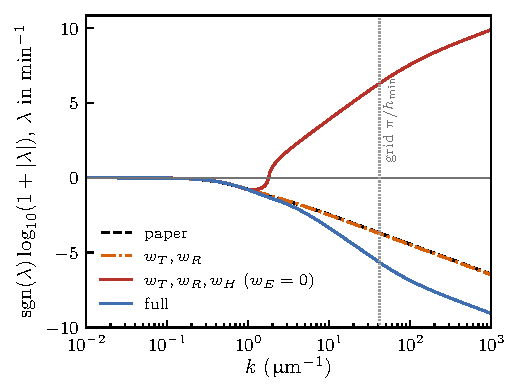
\includegraphics[width=0.55\linewidth]{figures/dispersion.pdf}
  \caption{Largest growth rate $\lambda$ of plane-wave perturbations of the uniform nematic
    state against the wavenumber $k$, maximized over the direction of $\mathbf k$, for the
    bare parameters of the paper ($B=9\times10^4$, finite). The rates are plotted as
    $\mathrm{sgn}(\lambda)\log_{10}(1+|\lambda|)$. Dashed: the paper's model; dash-dotted:
    exact moments in the self-propulsion and rotational-friction terms; red: in addition the
    \upd{$\nabla\H$ terms} with the lowest-order mobility ($w_E=0$); blue: the full model. The dotted
    line marks $\pi/h_\mathrm{min}$ of the solver grid. Script: \texttt{dispersion.py}.}
  \label{fig:dispersion}
\end{figure}

\Cref{fig:dispersion} checks this on the linearized continuum equations about the uniform
state, independently of the solver. In the model with $w_H=1$ and $w_E=0$, perturbations
with $k>1.8~\micron^{-1}$ grow, and the rate increases without bound with $k$. Finite $B$ does
not cure it: once $k^2\gg B/K$ the density stops following $\Q$, but the $2\times2$
density--amplitude block then has a negative determinant,
$\propto BKk^6(1-2S^2)/\xi_0^2$, so one eigenvalue stays positive and grows as
$(B/\xi_0)(2S^2-1)k^2$. In the full model all perturbations decay, and the fourth-order
coefficient of the amplitude mode is $-(K/\xi_0)(1-2S^2+g_2S^2)=-0.18~\micron^4/\minute$
at the far-field order. The paper's model, without $\nabla\H$, is stable too.

The closure and the $\nabla\H$ terms are therefore not independent choices. The paper's
combination, lowest-order closure without $\nabla\H$, is consistent. Keeping $\nabla\H$
requires the exact moments, at least in the elastic mobility. In the continuation below we
therefore switch $w_H$ and $w_E$ on together.

\subsection*{The far field}
With the bare parameters of the paper fixed, the exact moments also change the ordered state
far from the defect. In a uniform nematic only the rotational friction and the rotational
diffusion survive in \cref{eq:ss-Q}, and with $h=-(a+2bS^2)S$ they balance when
\begin{equation}
  \label{eq:Sinf}
  -\bigl(a+2bS^2\bigr)\bigl(1-w_Rg_2S^2\bigr)=\Lambda\xir .
\end{equation}
At $w_R=0$ this gives the paper's $S_0=\sqrt{-a'/(2b)}=0.90$. The exact moment
$\la\hat\Q'\hat\Q'\ra_\varrho$ weakens the ordering drive of the molecular field by the factor
$1-g_2S^2=1-\la\cos4(\theta-\theta_0)\ra$. A rod aligned with the director only turns the
director when it rotates; only misaligned rods change the degree of order, and their weight
falls as the order grows. The rotational diffusion $-4\Lambda\Q$, by contrast, is exact and
unchanged. The same noise then
disorders the rods more, and \cref{eq:Sinf} gives $S_\infty=0.846$ at $w_R=1$. We keep the bare
parameters, as in the paper's table, so the full model describes a slightly less ordered
monolayer than the paper's. At the wall the full solution has $S=\numSwallPxFull$--$\numSwallMxFull$.

% ======================================================================
\section{Numerical method}
\label{sec:numerics}

We want the new terms to be the only difference from the paper's steady state, so the solver
(\texttt{comoving\_defect\_full/}) keeps everything else of the paper's solver: the box
$[-20,20]^2~\micron^2$, the tensor grid graded by the Pad\'e profile (spacing
$0.075~\micron$ at the core and $1.96~\micron$ at the wall, $101^2$ nodes at refinement~1),
the fourth-order difference matrices with $\partial_y^2$ averaged with its mirror image, the
reservoir wall $\rho=1$, the free wall $\nh\cdot\nabla\Q=0$, the core pins
$Q_1(0,0)=Q_2(0,0)=0$ with $\u$ as their multipliers, and the mirror line $Q_2(x,0)=0$.
With all weights zero the discrete $(\rho,\Q)$ problem is then the paper's, node for node.

\subsection{Mixed formulation}
Rather than discretize $\nabla^4\Q$, we keep the molecular field
as an unknown, as one does for the Cahn--Hilliard equation. The unknowns are $\rho-1$,
$Q_1$, $Q_2$, $H_1$ and $H_2$ at every node, $51\,005$ values on the $101^2$ grid, plus
$u_x$ and $u_y$. We solve for $\rho-1$ rather than $\rho$ because only derivatives of $\rho$
enter at this order, and $(B/\xi_0)\nabla^2\rho$ evaluated on $\rho\approx1$ cancels numbers
of order one multiplied by $(B/\xi_0)/h^2$. That left a round-off floor of $10^{-9}$ in the
residual; with $\rho-1$ it is $10^{-12}$. Each of \cref{eq:ss-rho,eq:ss-Q,eq:ss-H} is then second order, and the fourth-order
structure enters only through their coupling. The principal parts use the compact
Laplacian through $\nabla\!\cdot\!(c\nabla f)=c\nabla^2f+\nabla c\cdot\nabla f$, because a
product of two first-derivative matrices on a collocated grid does not damp the shortest
wave. Only the term $\nabla\!\cdot\!(q\nabla\rho)$ keeps the divergence form of the paper's
solver.

\subsection{Walls}
The extra derivative needs one more wall condition. We take
$\nh\cdot\nabla\H=0$: no elastic flux of $\Q$ crosses the wall, and the elastic force has no
normal component there. Together with $\nh\cdot\nabla\Q=0$ it is the same as
$\nh\cdot\nabla\nabla^2\Q=0$. On the wall nodes the rows of the three equations are replaced
by $\rho=1$, $\nh\cdot\nabla\Q=0$ and $\nh\cdot\nabla\H=0$, with the signed normal summed at
the corners as in the paper's solver.

\subsection{Mirror line}
The line $Q_2(x,0)=0$ fixes the orientation of the defect. For a
second-order equation it is also the condition of odd symmetry, but a fourth-order equation
needs $\partial_y^2Q_2=0$ as well, which on the line is $H_2=0$. We therefore impose
$Q_2=H_2=0$ on the row $y=0$, the core node excepted, in place of the $Q_2$ equation and of
the $H_2$ definition. Both replaced rows hold anyway in the mirror-symmetric solution.
Without $H_2=0$, the Jacobian at full weights has a near-null mode in $Q_2$, $H_2$ and $u_y$.
Its smallest singular value is $2.3\times10^{-7}$, and $1.6\times10^{-5}$ once $H_2=0$ is
imposed (both with the scaling below; script \texttt{conditioning.wls}).

\subsection{Scaling}
At leading order $B$ enters only through the pressure $B(\rho-1)$, so the
columns of the Jacobian that belong to $\rho$ are larger than the others by a factor of order
$B$. We scale them by $\xi_0/B$, which makes the unknown the pressure $B(\rho-1)/\xi_0$, and
then equilibrate the rows. On the production grid this raises the smallest singular value of
the row-equilibrated Jacobian by a factor of $700$ to $4600$, for example from
$1.0\times10^{-8}$ to $1.6\times10^{-5}$ in the full model (\texttt{conditioning.wls}), and
the Newton step is measured in these scaled unknowns.

\subsection{Newton and continuation}
The Jacobian is exact. Each complex equation is
linearized in Wirtinger form, $\delta F=A\,\delta q+B\,\delta\bar q$, and the pair $(A,B)$
becomes the real $2\times2$ block
$\bigl(\begin{smallmatrix}\mathrm{Re}(A+B)&-\mathrm{Im}(A-B)\\ \mathrm{Im}(A+B)&\mathrm{Re}(A-B)\end{smallmatrix}\bigr)$.
It is refactorized at every Newton iteration, and Newton stops when the scaled step falls
below $10^{-10}$ or the equilibrated residual below $10^{-13}$. The steady state is reached by continuation. We first ramp $\zeta$ from $0$ to
$12.5$ in five steps at zero weights, as the paper's solver does. Then we move in weight space
along straight segments, starting with steps of $0.1$, doubling the step after an easy solve
and halving it after a failed one, with a secant predictor. Three paths end at the full
model:
\begin{itemize}
  \item path A: paper $\to w_T\to w_R\to(w_H,w_E)$, i.e.\ through
    $(w_T,w_R,w_H,w_E)=(0,0,0,0)$, $(1,0,0,0)$, $(1,1,0,0)$ and $(1,1,1,1)$;
  \item path B: paper $\to w_R\to(w_H,w_E)\to w_T$, through $(0,1,0,0)$ and $(0,1,1,1)$;
  \item path C: the $\zeta$ ramp directly at full weights.
\end{itemize}
Path A passes through the two models of the drift study, path B switches on \upd{the $\nabla\H$
terms} before the self-propulsion term, and the three together test whether the full solution
depends on the way it is reached. On the finer grids of the convergence test we start instead
from the refinement-1 solution, interpolated onto the new grid, and polish it with Newton.

% ======================================================================
\section{Validation}
\label{sec:validation}

Before we interpret the full solution we check that the solver reproduces what is already
known and that its answer does not depend on how it is reached. \Cref{tab:validation}
collects the checks. The Jacobian agrees with central differences of the residual in every
block. With all weights zero the solver gives the paper's drift velocity to $10^{-10}$, and
with $w_T$ and $w_R$ switched on it gives the two values of the drift study, which were computed
with an independent modification of the paper's solver. The state stays mirror symmetric to
round-off, so $u_y$ and the force that the mirror line exerts vanish. The three paths end at the same
full solution, to all printed digits. At $\zeta=0$ the full model has no active
force, and the defect should be static. The residual drift is a discretization error: it
falls by $5.7$ between refinements~1 and~1.5, as $h^4$ does ($1.5^4=5.1$).

\begin{table}[t]
  \centering
  \caption{Checks of the solver. Box half-width $20~\micron$, refinement~1 ($101^2$
    nodes) unless stated. References: the paper's steady state (meta file of the
    $B=9\times10^4$ fluctuation run) and the drift study (\texttt{app:drift};
    \texttt{claude\_experiments/drift\_closure\_2026\_10\_09/summary.json}).
    Scripts: \texttt{comoving\_defect\_full/check\_jacobian.wls} and
    \texttt{run\_full.wls}.}
  \label{tab:validation}
  \small
  \begin{tabular}{lll}
    \toprule
    check & reference & result\\
    \midrule
    Jacobian vs.\ central differences, all blocks & -- & max.\ rel.\ error $\numjacWorst$\\
    paper's model, $u_x$ ($\micron/\minute$) & $0.2384998$ & $\numuFineAOnePZero$\\
    $+w_T$ & $-0.1378980$ & $\numuFineAOnePOne$\\
    $+w_T,w_R$ & $-0.1964310$ & $\numuFineAOnePTwo$\\
    mirror symmetry, full model: $|u_y|$, line force & 0 & $\numuyAOneFull$, $\numlfAOneFull$\\
    full model via path A / B / C & equal & $\numuFineAOneFull$ / $\numuFineBOneFull$ / $\numuFineCOneFull$\\
    $\zeta=0$, full weights: $u_x$ at refinement 1 / 1.5 & 0 &
      $\numuSciZOneFull$ / $\numuSciZOneHalfFull$\\
    far-field order at the wall, full model & $S_\infty=\numSInfUniform$ & $\numSwallPxFull$--$\numSwallMxFull$\\
    \bottomrule
  \end{tabular}
\end{table}

% ======================================================================
\section{Results}
\label{sec:results}
\subsection{Drift velocity}
In the drift study the closure decided the direction in which the defect moves, so we first
ask whether the full model keeps that direction. \Cref{fig:upath} follows $u_x$ along paths
A and B, and \cref{tab:drift} lists it at the milestones.

\begin{table}[t]
  \centering
  \caption{Drift velocity $u_x$ of the $+1/2$ defect ($\micron/\minute$; positive toward
    the tail, negative toward the head) for the models along the continuation paths. Box
    half-width $20~\micron$, refinement~1.}
  \label{tab:drift}
  \small
  \begin{tabular}{llc}
    \toprule
    model & $(w_T,w_R,w_H,w_E)$ & $u_x$\\
    \midrule
    paper & $(0,0,0,0)$ & $\numuAOnePZero$\\
    $+$ self-propulsion term & $(1,0,0,0)$ & $\numuAOnePOne$\\
    $+$ rotational friction & $(1,1,0,0)$ & $\numuAOnePTwo$\\
    full & $(1,1,1,1)$ & $\numuAOneFull$\\
    \midrule
    rotational friction only & $(0,1,0,0)$ & $\numuBOneBwR$\\
    $+$ \upd{$\nabla\H$ terms} & $(0,1,1,1)$ & $\numuBOneBwRH$\\
    \midrule
    \upd{$\nabla\H$ terms}, lowest-order mobility & $(1,1,w_H,0)$ & continuation stops at $w_H=\numwHmaxLow$\\
    \bottomrule
  \end{tabular}
\end{table}

\begin{figure}[t]
  \centering
  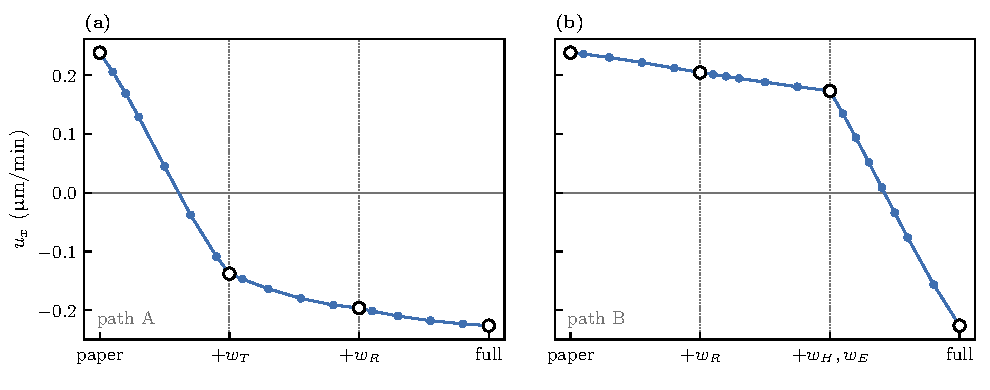
\includegraphics[width=\linewidth]{figures/u_path.pdf}
  \caption{Drift velocity along the continuation paths, at every converged step (small
    markers) and at the milestones (open circles). \textbf{(a)} Path A: the weights $w_T$,
    $w_R$ and then $(w_H,w_E)$ go from $0$ to $1$. \textbf{(b)} Path B: $w_R$, then
    $(w_H,w_E)$, then $w_T$. Both end at the full model. Box half-width $20~\micron$,
    refinement~1.}
  \label{fig:upath}
\end{figure}

Along path A, the fourth harmonic of the self-propulsion term reverses the drift, from
$\numuAOnePZero$ to $\numuAOnePOne~\micron/\minute$, as in the drift study. The exact rotational
friction then moves the defect faster toward its head, to $\numuAOnePTwo$, and the
\upd{$\nabla\H$ terms bring} it to the full value $\numuAOneFull~\micron/\minute$. Path B switches
the terms on in a different order. The rotational friction alone slows the drift toward the
tail to $\numuBOneBwR$, and \upd{the $\nabla\H$ terms slow} it further to $\numuBOneBwRH$, but
neither reverses it. Only the self-propulsion term does, and it brings the drift to the same
full value. Path C, the $\zeta$ ramp at full weights, ends there as well. Each term
changes $u_x$ by about the same amount whichever order it comes in: the self-propulsion term
by $-0.38$ to $-0.40~\micron/\minute$, the rotational friction by $-0.03$ to $-0.06$, and
\upd{the $\nabla\H$ terms} by $-0.03$. The full model therefore keeps the conclusion of the drift study: the
defect moves toward its head, and the term that sets the direction is the fourth harmonic of
the self-propulsion term. \upd{The $\nabla\H$ terms make} the defect about $15\%$ faster.

With the lowest-order mobility, $w_E=0$, the continuation of \upd{the $\nabla\H$ terms} stops at
$w_H=\numwHmaxLow$, where Newton no longer converges however small the step. This is the
ill-posedness of \cref{sec:wellposed}.

\subsection{Size of the box and resolution}
\begin{figure}[t]
  \centering
  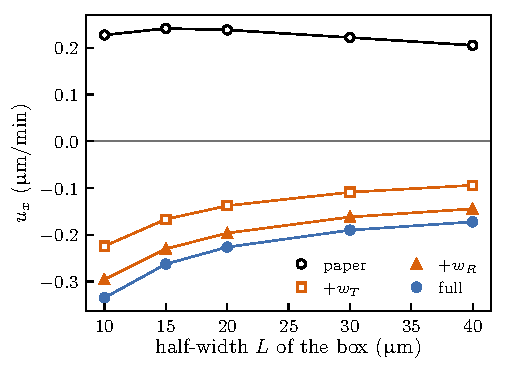
\includegraphics[width=0.55\linewidth]{figures/u_box.pdf}
  \caption{Drift velocity against the half-width $L$ of the box, for the paper's model, the
    two intermediate models of path A and the full model. Refinement~1.}
  \label{fig:ubox}
\end{figure}
As in the paper's model, the drift velocity depends on the size of the box
(\cref{fig:ubox}), because the far field of the defect, which the wall cuts off, contributes
to it (\texttt{app:drift}). With full weights the defect moves toward its head in every box, at
$\numuLTenFull$, $\numuLFifteenFull$, $\numuAOneFull$, $\numuLThirtyFull$ and
$\numuLFortyFull~\micron/\minute$ for $L=10$, $15$, $20$, $30$ and $40~\micron$.
The full solution is also resolved on the grid of the paper. Refining the grid by $1.5$ and
$2$ changes the full $u_x$ from $\numuFineAOneFull$ to $\numuFineFOneHalfFull$ and
$\numuFineFTwoFull~\micron/\minute$, and fourth-order extrapolation gives
$\numuExtrap~\micron/\minute$. The refinement-1 value is thus off by
$\numuErrOne~\micron/\minute$ ($\numuErrOneRel\%$), far less than the differences between
the models. The paper's model gives $\numuFineAOnePZero$, $\numuFineAOneHalfPZero$ and
$\numuFineGTwoPZero$ on the three grids. The two finer grids
were reached by interpolating the refinement-1 solution and polishing it with Newton,
because the continuation through small $w_H$ becomes fragile on finer grids: there the
fourth-order term is a singular perturbation, with boundary layers at the walls thinner than
the wall cells.

\subsection{Structure of the defect}
\begin{figure}[t]
  \centering
  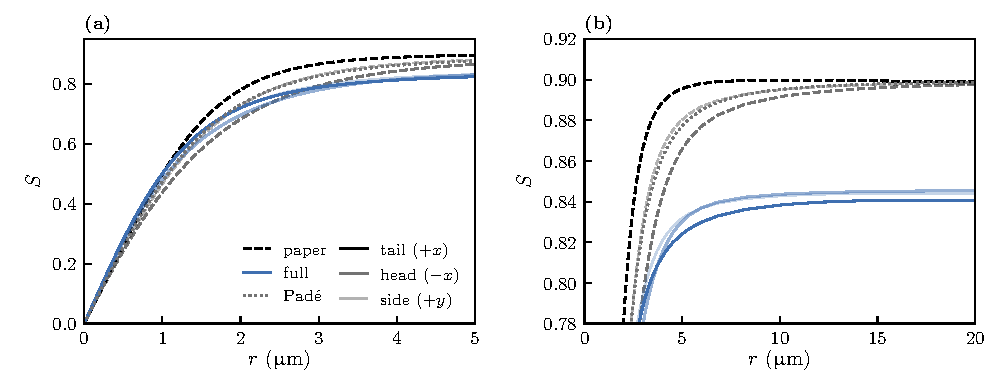
\includegraphics[width=\linewidth]{figures/S_axes.pdf}
  \caption{Strength $S$ of the nematic order along the axis of the defect, on the tail side
    ($+x$, dark) and the head side ($-x$, faded), and across it ($+y$, light), for the
    paper's model (black, dashed) and the full model (blue), with the Pad\'e profile of the
    paper (dotted). \textbf{(a)} The core. \textbf{(b)} The whole box.}
  \label{fig:Saxes}
\end{figure}

\begin{figure}[t]
  \centering
  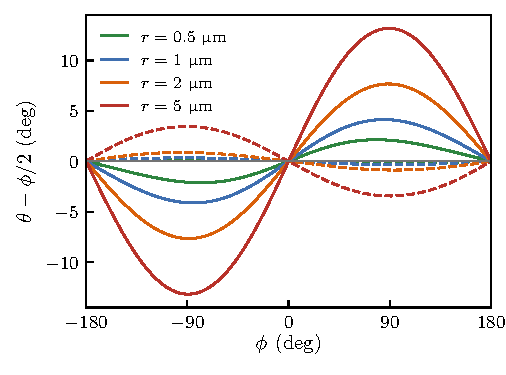
\includegraphics[width=0.48\linewidth]{figures/director_dev.pdf}\hfill
  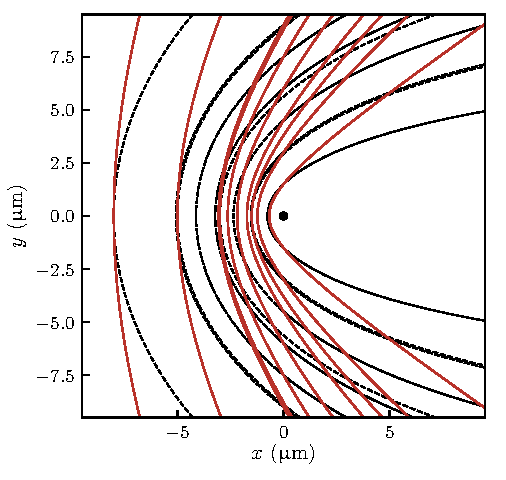
\includegraphics[width=0.48\linewidth]{figures/director_lines.pdf}
  \caption{\textbf{Left:} deviation of the director angle from the ideal $+1/2$ profile,
    $\theta-\phi/2$, against the polar angle $\phi$ on circles of radius $0.5$, $1$, $2$ and
    $5~\micron$; dashed: paper, solid: full. \textbf{Right:} director lines of the paper's
    model (black, dashed) and of the full model (red).}
  \label{fig:director}
\end{figure}

The full model changes the defect in three ways (\cref{fig:Saxes,fig:director,fig:maps}). The far
field is less ordered, $S=\numSwallFull$ at the wall against $\numSwallPaper$, as the
uniform balance \cref{eq:Sinf} predicts. The core is smaller: $S$ reaches half its far-field
value at $\numrhalfTailFull$, $\numrhalfHeadFull$ and $\numrhalfSideFull~\micron$ along the tail,
the head and the side, against $\numrhalfTailPaper$, $\numrhalfHeadPaper$ and
$\numrhalfSidePaper~\micron$ in the paper's model. This comes from \upd{the $\nabla\H$ terms}: with
$w_T$ and $w_R$ alone the half radii are still $\numrhalfTailPlusR$--$\numrhalfHeadPlusR~\micron$. Near the core,
where $S$ is small, the elastic flux contributes $(a/\xi_0)\nabla^2\Q-(K/\xi_0)\nabla^4\Q$
to the $\Q$ equation. With $a<0$ the first part opposes the elastic relaxation
$(4K'/\xir)\nabla^2\Q$ and cancels $|a|\xir/(4\xi_0K')=83\%$ of it there, which favors a
sharper core.
Finally, the director turns away from the ideal profile. The largest deviation of
$\theta-\phi/2$ is $\numdevFullROnepZero^\circ$, $\numdevFullRTwopZero^\circ$ and
$\numdevFullRFivepZero^\circ$ at $r=1$, $2$ and $5~\micron$, against
$\numdevPaperROnepZero^\circ$, $\numdevPaperRTwopZero^\circ$ and $\numdevPaperRFivepZero^\circ$
in the paper's model, and it has the opposite sign: on the side of the defect at
$\phi=90^\circ$ the paper's director turns clockwise from the ideal profile, the full one
counterclockwise. This deviation comes from the self-propulsion term: with $w_T$ alone it
is already $\numdevPlusTROnepZero^\circ$, $\numdevPlusTRTwopZero^\circ$ and
$\numdevPlusTRFivepZero^\circ$, as the drift study found.

\subsection{Density and forces}
\begin{figure}[t]
  \centering
  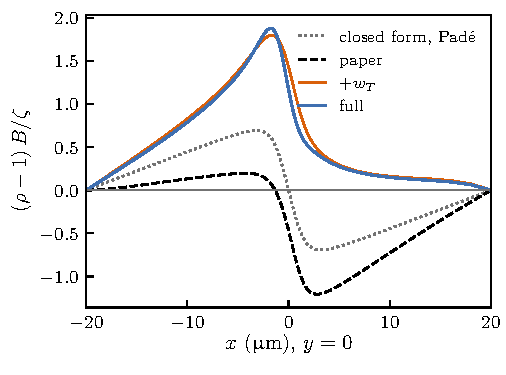
\includegraphics[width=0.55\linewidth]{figures/rho_axis.pdf}
  \caption{Density along the axis, $(\rho-1)B/\zeta$, for the paper's model, with the
    self-propulsion term ($+w_T$), and for the full model, with the closed form of the paper on
    the Pad\'e profile (dotted).}
  \label{fig:density}
\end{figure}

\begin{figure}[t]
  \centering
  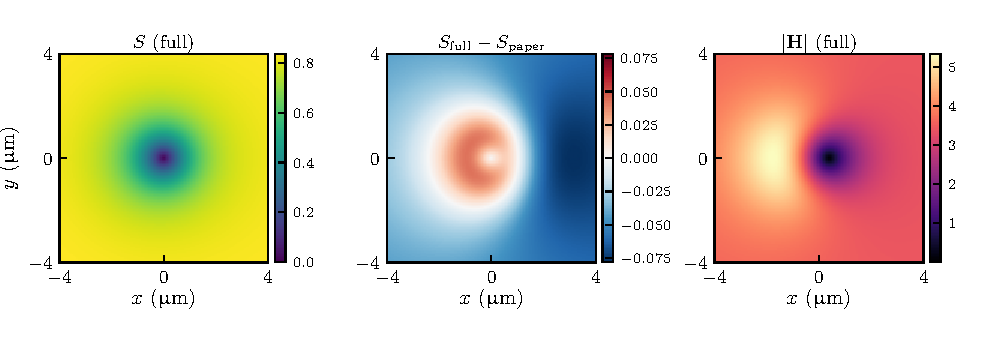
\includegraphics[width=\linewidth]{figures/maps.pdf}
  \caption{Near the core of the full model: the order $S$, its change from the paper's model,
    and the magnitude of the molecular field $|\H|$.}
  \label{fig:maps}
\end{figure}

\begin{figure}[t]
  \centering
  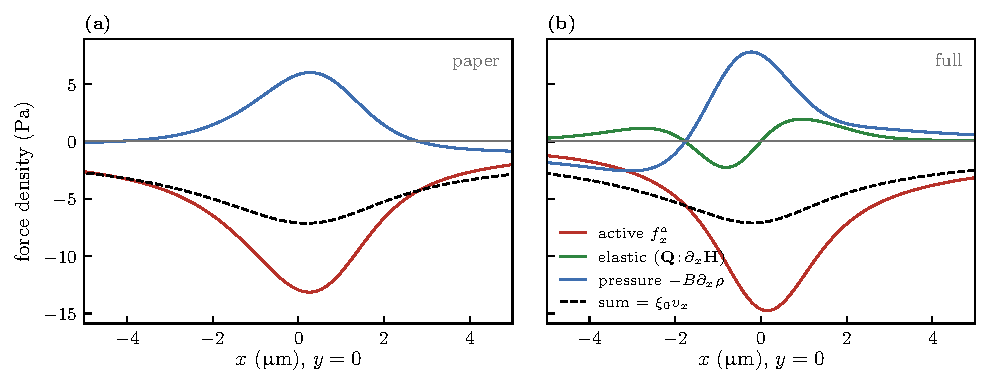
\includegraphics[width=\linewidth]{figures/forces_axis.pdf}
  \caption{Force densities along the axis that enter the density flux,
    $\xi_0\bm v=-B\nabla\rho+\Q\!:\!\nabla\H+\bm f^a$: the active force, the pressure
    gradient and, in the full model, the elastic force; dashed: their sum.
    \textbf{(a)} The paper's model. \textbf{(b)} The full model.}
  \label{fig:forces}
\end{figure}

The density still departs from one only at order $\zeta/B$, but its shape changes
(\cref{fig:density}). In the paper's model $(\rho-1)B/\zeta$ lies between $\numrhoMinPaper$
and $\numrhoMaxPaper$, so the defect mostly depletes the monolayer. In the full model it lies
between $\numrhoMinFull$ and $\numrhoMaxFull$, so the defect compresses it, most strongly
about $2~\micron$ from the core on the head side. Again the self-propulsion term does
most of this: with $w_T$ alone the range is already $\numrhoMinPlusT$ to
$\numrhoMaxPlusT$. The density equation does not contain $w_T$, so the change comes from the
deformed nematic field, through the active force $-\zeta\nabla\!\cdot\!\Q$. Even the largest
value, $\numrhoMaxFull\,\zeta/B\approx2.6\times10^{-4}$, stays two orders of magnitude below
the standard deviation of the density fluctuations, $1.9\%$ in the manuscript.

\Cref{fig:forces} shows the forces that drive the density flux along the axis. The elastic
force of the full model reaches $\numfElasticMaxFull$~Pa near the core, against
$\numfActiveMaxFull$~Pa for the active force, so it is a correction of about $15\%$. At the
core the three forces sum to $\numfNetCoreFull$~Pa in the full model and to
$\numfNetCorePaper$~Pa in the paper's model. The cells at the core therefore move toward the
head at the same speed in both models, $1.4~\micron/\minute$ in the laboratory frame.

% ======================================================================
\section{Density fluctuations}
\label{sec:fluct}

The paper computes the equal-time density variance around the comoving defect from the
linearization of its reduced model (\texttt{app:lyapunov}). We now repeat that calculation
for the full model, with the same parameters, box, wall and short-length cutoff, and we
split the variance into the contributions of the separate noise sources and of the two
routes by which noise reaches the density. The aim is to see whether the closure and the
$\nabla\H$ terms, which reverse the drift, also change the variance profile that the paper
connects to layer formation.

\subsection{Linearized stochastic model}
The noise of the full model is that of the manuscript (\texttt{app:dean-angle},
eq.~Q-noise-correlators). The reversal noise of the rods drives one flux that carries both
density and alignment, $\bm\eta_\rho$ in the density equation and $\bm\eta^{\Q}$ in the $\Q$
equation, and its covariances contain $\Q$, $\la\hat\Q\hat\Q\ra_\varrho$ and
$\la\hat\Q\hat\Q\hat\Q\ra_\varrho$. The rotational noise enters the $\Q$ equation alone, as
the local term $\mathbf f^{\Q}$ with covariance $(2\Lambda/\rho_0)\la\hat\Q'\hat\Q'\ra_\varrho$,
and it is independent of the reversal noise. \upd{The $\nabla\H$ terms are} deterministic, so the
full model brings no new noise. The noise covariance is therefore the one the paper's solver
already builds from the exact moments, now evaluated on the full steady state.

The drift changes. We linearize \cref{eq:ss-rho,eq:ss-Q,eq:ss-H} about the full steady state
in the comoving frame, $\psi=(\delta\rho,\delta Q_1,\delta Q_2)$, and eliminate $\delta h$,
\begin{equation}
  \delta h=-(a+4b|q|^2)\,\delta q-2bq^2\,\delta\bar q+K\nabla^2\delta q .
\end{equation}
The density row gains $-(2w_H/\xi_0)\,\mathrm{Re}\,\nabla\!\cdot\!(\delta q\nabla\bar h+q\nabla\delta\bar h)$,
the coupling of the density to the order through the elastic force, and the $\Q$ rows gain
\begin{equation}
  \frac{\zeta w_T}{2\xi_0}\dbar^2\delta C-\frac{4w_R}{\xir}\bigl(\delta C\,\bar h+C\,\delta\bar h\bigr)
  -\frac{w_H}{\xi_0}\Bigl[\nabla^2\delta h+w_E\nabla\!\cdot\!\bigl(\delta C\,\nabla\bar h+C\,\nabla\delta\bar h\bigr)\Bigr],
\end{equation}
with $\delta C=(2g_2q+g_2'|q|^2q)\,\delta q+g_2'q^3\,\delta\bar q$ and $g_2'=\mathrm d g_2/\mathrm d|q|^2$.
All other terms of the drift, including the advection by $\u+(B/\xi_0)\nabla\rho_\mathrm{ss}$, are the
paper's. With all weights zero the drift is the paper's operator.

We solve the Lyapunov equation $\mathbf A\mathbf C+\mathbf C\mathbf A^{\mathsf T}+W\mathbf N W=0$
on the paper's uniform grid in the box $[-20,20]^2~\micron^2$ with the reservoir wall $\psi=0$
(\texttt{app:lyapunov-walls}). Since $\delta h$ is formed with the same Dirichlet Laplacian,
the wall also has $\delta\H=0$. The noise is smoothed by $W=\exp(\ell_W^2\nabla^2/4)$ with the
calibrated $\ell_W$ of the paper (eq.~ell-eff), so that the pedestal is
$\Sigma_\mathrm{ped}=\zeta/(2\pi B\rho_0\ell_\mathrm n^2)=\nfped$ at $\ell_\mathrm n=0.5~\micron$.
We write $\nu=\mathrm{Var}\,\delta\rho/\Sigma_\mathrm{ped}-1$ and $\nu_0$ for its maximum on the
axis.

\subsection{Splitting the variance}
The variance is linear in the noise covariance, so a split of $\mathbf N$ splits $\mathbf C$
exactly. We use five pieces:
\begin{itemize}
  \item from the reversal noise, the isotropic part $\rho\,\delta_{ij}$ of the density
    covariance (the pedestal), its anisotropic part $Q_{ij}$, the cross covariance of
    $\bm\eta_\rho$ and $\bm\eta^{\Q}$, and the covariance of $\bm\eta^{\Q}$;
  \item the rotational noise $\mathbf f^{\Q}$.
\end{itemize}
The first four belong to one physical flux and need not be positive separately; only their
sum and the rotational piece are covariances.

The second split follows the route by which the noise reaches the density. We write
$\delta\rho=\delta\rho_\mathrm d+\delta\rho_{\Q}$, where $\delta\rho_\mathrm d$ obeys the density
equation with $\delta\Q$ frozen, $\partial_t\delta\rho_\mathrm d=(B/\xi_0)\nabla^2\delta\rho_\mathrm d
-\nabla\!\cdot\!\bm\eta_\rho$. This is the paper's analytic model on the lattice, and
$\delta\rho_{\Q}$ is the density that the fluctuating order drives. Then
\begin{equation}
  \mathrm{Var}\,\delta\rho=\mathrm{Var}\,\delta\rho_\mathrm d+\mathrm{Var}\,\delta\rho_{\Q}
  +2\,\mathrm{Cov}(\delta\rho_\mathrm d,\delta\rho_{\Q}).
\end{equation}
$\mathrm{Var}\,\delta\rho_\mathrm d$ needs only the density block, which the sine basis
diagonalizes, and $\mathrm{Cov}(\delta\rho_\mathrm d,\psi)$ solves the Sylvester equation
$\mathbf A_{\rho\rho}\mathbf X+\mathbf X\mathbf A^{\mathsf T}+(W\mathbf NW)_{\rho\cdot}=0$.

\subsection{Numerics and validation}
The new solver (\texttt{lyapunov\_full/}) assembles the drift and the five noise pieces in
Mathematica and reuses the grid, the closure and the cutoff of the paper's module, which it
loads unchanged. A Python backend computes one real Schur factorization $\mathbf A=Z T Z^{\mathsf T}$
and uses it for every right-hand side. It moves the smoothing onto the Schur vectors,
$Z^{\mathsf T}W\mathbf N_kWZ=(WZ)^{\mathsf T}\mathbf N_k(WZ)$, so that no dense noise matrix is formed,
and the same factor solves the Sylvester equation of the pathway split. The total is refined
once, as in the paper's backend, and the five pieces keep only the diagonals of the six
blocks of $\mathbf C$. \Cref{tab:fluct-validation} lists the checks.

\begin{table}[t]
  \centering
  \caption{Checks of the fluctuation solver. Small-grid checks at $N_\mathrm{int}=41$
    (\texttt{lyapunov\_full/check\_small.wls}, \texttt{check\_multi.py},
    \texttt{check\_linearization.wls}; logs in \texttt{lyapunov\_full/logs/}). Production:
    $N_\mathrm{int}=\nfN$, $\Delta x=\nfh~\micron$.}
  \label{tab:fluct-validation}
  \small
  \begin{tabular}{p{0.6\linewidth}l}
    \toprule
    check & result\\
    \midrule
    paper's model: drift / smoothed noise against the paper's module & $\nfchkA$ / $\nfchkQ$\\
    backend against the module's eigen-solver, paper / full model & $\nfchkCP$ / $\nfchkCF$\\
    each noise piece against a separate dense solve & $\le\nfchkSrcP$\\
    pathway split against the augmented system $(\delta\rho_\mathrm d,\psi)$ & $\nfchkVdP$\\
    new drift terms against the symbolic Gateaux derivative, $N_\mathrm{int}=41,81,161$ & $\nflinA$, $\nflinB$, $\nflinC$\\
    paper's model against the paper's runs, $N_\mathrm{int}=150$ / $180$ (max.\ $|\Delta\nu|$) & $\nfrefDiffA$ / $\nfrefDiffB$\\
    sum of the five pieces against the total, $\rho\rho$ diagonal, paper / full & $\nfsrcsumPaper$ / $\nfsrcsumFull$\\
    Lyapunov residual (refined), paper / full & $\nfresPaper$ / $\nfresFull$\\
    largest $\mathrm{Re}\,\lambda$, paper / full (min$^{-1}$) & $\nfmaxRePaper$ / $\nfmaxReFull$\\
    \bottomrule
  \end{tabular}
\end{table}

The new drift terms are checked against the continuum: for a smooth texture and a smooth
direction, $\mathbf A\psi$ converges to the symbolic derivative of the full equations at second
order in the grid spacing. With all weights zero the solver gives the paper's runs at
$N_\mathrm{int}=150$ and $180$ to round-off. Both models are stable on this grid. On coarser grids the full
model is not: its largest eigenvalue is positive at $N_\mathrm{int}\le120$ and falls quickly with
refinement, as the paper's does.

\subsection{The variance near the defect}
\begin{figure}[t]
  \centering
  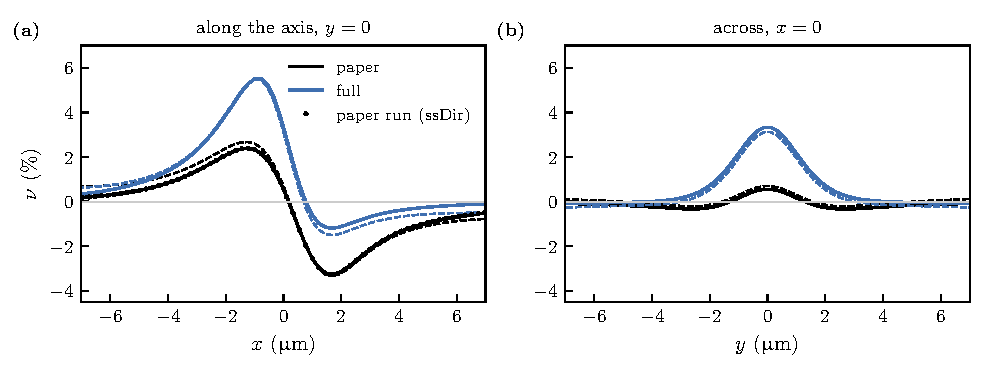
\includegraphics[width=\linewidth]{figures/fluct_axis.pdf}
  \caption{Relative density variance $\nu$ along the axis (a) and across it through the core (b),
    $N_\mathrm{int}=\nfN$. Solid: Lyapunov solution; dashed: the paper's analytic formula
    (eq.~total-gauss) evaluated on the same steady state; dots: the paper's run
    (ssDir, same grid), which the solver reproduces.}
  \label{fig:fluct-axis}
\end{figure}

\begin{figure}[t]
  \centering
  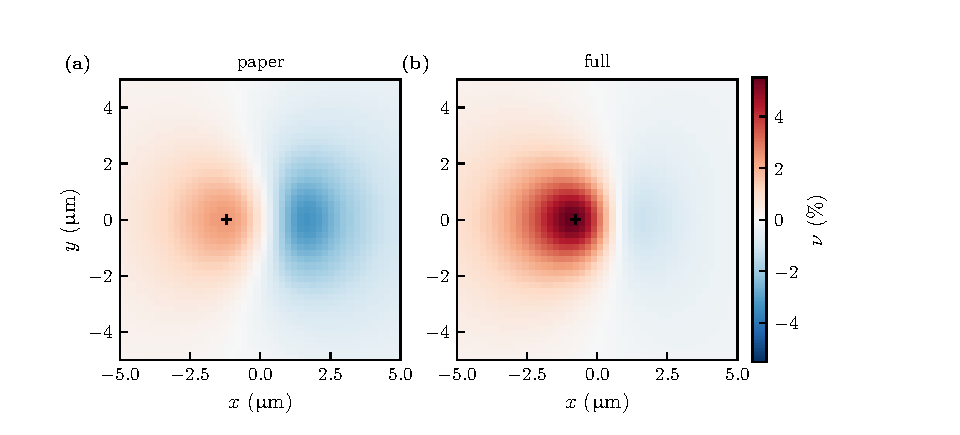
\includegraphics[width=0.9\linewidth]{figures/fluct_maps.pdf}
  \caption{$\nu$ near the core, paper (a) and full model (b), same color scale; $+$ marks the
    maximum.}
  \label{fig:fluct-maps}
\end{figure}

The full model more than doubles the modulation of the variance
(\cref{fig:fluct-axis,fig:fluct-maps}). Along the axis the maximum rises from
$\nu_0=\nfnuPaper\%$ to $\nfnuFull\%$ and moves toward the core, from
$x=\nfxPaper$ to $\nfxFull~\micron$, while the minimum on the head side becomes shallower,
$\nfnuMinFull\%$ instead of $\nfnuMinPaper\%$. Across the axis the variance at the core rises
from $\nfnuCrossPaper\%$ to $\nfnuCrossFull\%$. The paper's analytic formula, evaluated on
each steady state, gives the same change, $\nfnuAnPaper\%$ and $\nfnuAnFull\%$, so the change
comes from the steady state and not from the new fluctuation dynamics. That formula
convolves $\partial_i\partial_jQ^\mathrm{ss}_{ij}$ with a kernel of range $\ell_\mathrm n$, and the
full steady state has the sharper core and the turned director of \cref{sec:results}.

\begin{figure}[t]
  \centering
  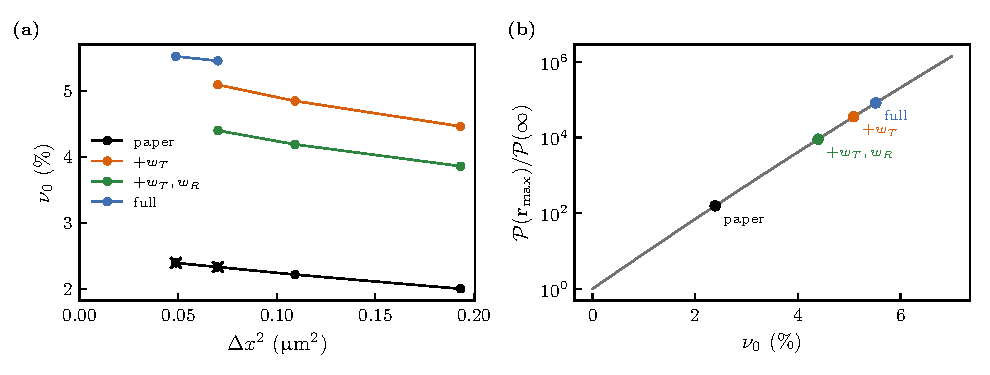
\includegraphics[width=\linewidth]{figures/fluct_ladder.pdf}
  \caption{(a) $\nu_0$ against the squared grid spacing for the models of path~A; crosses:
    the paper's runs at $N_\mathrm{int}=150$ and $180$. (b) The enhancement of eq.~R-value,
    $\exp[(z_\infty^2/2)\nu_0/(1+\nu_0)]$ with $z_\infty=20.8$, on the finest stable grid of
    each model.}
  \label{fig:fluct-ladder}
\end{figure}

The model ladder of \cref{fig:fluct-ladder} shows which term does it. The fourth harmonic
of the self-propulsion term alone gives $\nu_0=\nfnuWT\%$ (at $N_\mathrm{int}=\nfNWT$, where the paper's model gives
$\nfnuPaperLadder\%$), the rotational friction lowers it to $\nfnuWTR\%$, and \upd{the $\nabla\H$ terms}
\upd{raise} it again. The closure that reverses the drift therefore also sets the
variance. In every model $\nu_0$ still grows slowly with refinement; for the paper's model
it is $2.00$, $2.21$, $2.33$ and $2.39\%$ at $N_\mathrm{int}=90$, $120$, $150$ and $180$
(\texttt{data/fluct\_analysis.txt}), and for the full model $5.45$ and $5.52\%$ at $150$ and $180$.

The paper turns $\nu_0$ into the layering enhancement through eq.~R-value. Because $z_\infty^2/2=216$
amplifies the modulation, the enhancement goes from $\nfRPaper$ in the paper's model to
$\nfRFull$ in the full model with the same $z_\infty$. In the paper $z_\infty$ follows from the fit of $B$, and the resulting enhancement lies in the
first bin of the measured profile, $40$--$500$ around $2\times10^2$. With the full model's $\nu_0$ the
same enhancement would need $z_\infty\approx14$ instead of $20.8$, that is, a different fit of $B$. \Cref{fig:fluct-layering}
shows the circle-averaged profiles of eq.~p-layer-radial. Their shapes agree between the two
models: the profile about $\mathbf r_\mathrm{max}$ falls monotonically, and the one about the core
peaks off the core, at $r\simeq1~\micron$ instead of $1.5~\micron$.

\begin{figure}[t]
  \centering
  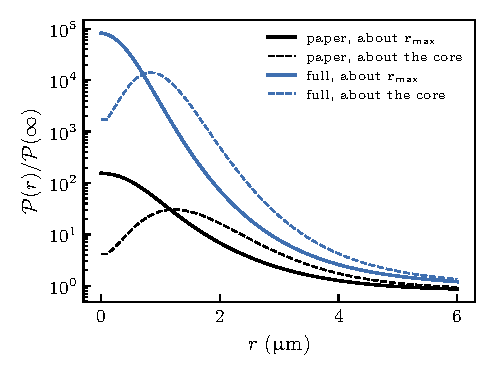
\includegraphics[width=0.5\linewidth]{figures/fluct_layering.pdf}
  \caption{Layering probability averaged over circles of radius $r$ (eq.~p-layer-radial)
    about $\mathbf r_\mathrm{max}$ (solid) and the core (dashed), $z_\infty=20.8$.}
  \label{fig:fluct-layering}
\end{figure}

\subsection{Where the variance comes from}
\begin{figure}[t]
  \centering
  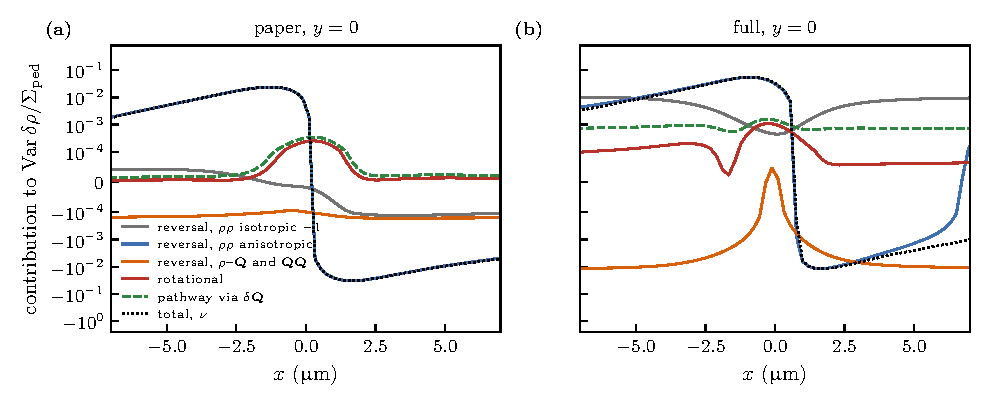
\includegraphics[width=\linewidth]{figures/fluct_sources.pdf}
  \caption{Contributions to $\mathrm{Var}\,\delta\rho/\Sigma_\mathrm{ped}$ along the axis
    (symmetric-log scale, linear below $10^{-4}$). Lines: the noise pieces (the isotropic
    one minus the pedestal; the two pieces of the alignment flux summed); dashed:
    $\mathrm{Var}\,\delta\rho_{\Q}$, the density driven by the fluctuating order; dotted: the
    total $\nu$, which coincides with the anisotropic piece.}
  \label{fig:fluct-sources}
\end{figure}

Almost all of the modulation comes from the anisotropic part of the reversal noise in the
density flux (\cref{fig:fluct-sources}): at the maximum it gives $\nfanisoPaper\%$ in the
paper's model and $\nfanisoFull\%$ in the full model, against $\nu_0=\nfnuPaper\%$ and
$\nfnuFull\%$. The pathway split says the same: the density with $\delta\Q$ frozen gives
$\nfpathDirectPaper\%$ and $\nfpathDirectFull\%$ above the pedestal at the maximum. The
fluctuating order adds $\mathrm{Var}\,\delta\rho_{\Q}=\nfpathQPaper\times10^{-4}$ of the pedestal
in the paper's model and $\nfpathQFull\times10^{-4}$ in the full model, and the interference
term is of the same size with the opposite sign. The rotational noise contributes
$\nfQQrotPaper\times10^{-4}$ and $\nfQQrotFull\times10^{-4}$. This confirms the paper's
argument that the density follows the order adiabatically. On the scale of the cutoff the
order relaxes at most at $4K'/(\xir\ell_\mathrm n^2)\approx20~\minute^{-1}$, while the density
relaxes within $\tau_c\approx0.4$~ms (eq.~tau-c), so the order acts
as a slowly varying force whose density response is of order $\zeta/B$.

\upd{The $\nabla\H$ terms make} the order matter ten times more (with $w_T$ and $w_R$ alone,
$\mathrm{Var}\,\delta\rho_{\Q}$ stays at $1\times10^{-4}$ on the grid $N_\mathrm{int}=150$), because it couples
$\delta\Q$ to the density flux through the elastic force as well as through the active one.
In the full model the density driven by the order makes up $\nfpathQFarFull\times10^{-4}$ of the
pedestal even far from the core. There the separate pieces of the reversal noise are
large but cancel: the density noise alone lifts the variance by $\nfisoFarFull\%$, through
the order it excites and the elastic force that pushes back, the cross covariance removes
$\nfcrossFarFull\%$, and the noise of the alignment flux adds $\nfQQrevFarFull\%$. The rods
that carry density also carry alignment, so only the sum of the four pieces is meaningful.

\subsection{Order and director fluctuations, and the wandering core}
\begin{figure}[t]
  \centering
  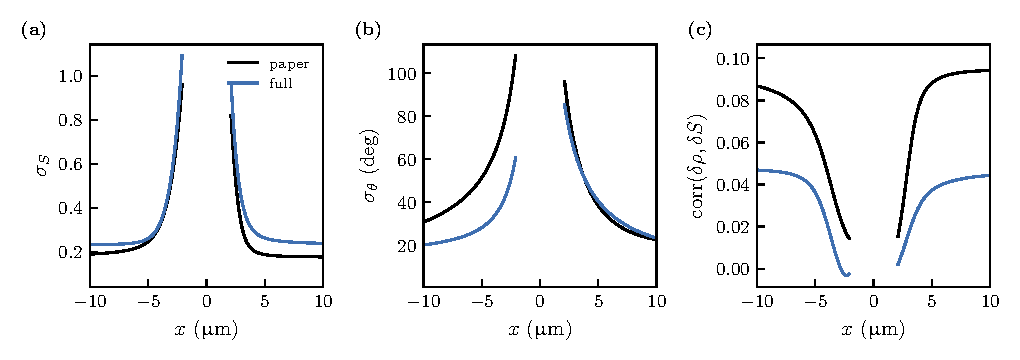
\includegraphics[width=\linewidth]{figures/fluct_nematic.pdf}
  \caption{Standard deviation of the order $S$ (a) and of the director angle (b), and the
    correlation coefficient of $\delta\rho$ and $\delta S$ (c), along the axis, outside
    $|x|<2~\micron$ where the translation mode dominates.}
  \label{fig:fluct-nematic}
\end{figure}

The order itself fluctuates strongly (\cref{fig:fluct-nematic}). Between $6$ and $10~\micron$
from the core the director angle has a standard deviation of $\nfsigTPaper^\circ$ in the
paper's model and $\nfsigTFull^\circ$ in the full model, and $S$ of $\nfsigSPaper$ and
$\nfsigSFull$. These numbers are large for a linear theory. The rotational noise supplies
about $\nfshareRotFull\%$ of the director variance there; the reversal noise supplies the
rest. Away from the core the density and the order are only weakly correlated, with a
correlation coefficient below $0.1$, which is why the order hardly enters the density variance.

\begin{figure}[t]
  \centering
  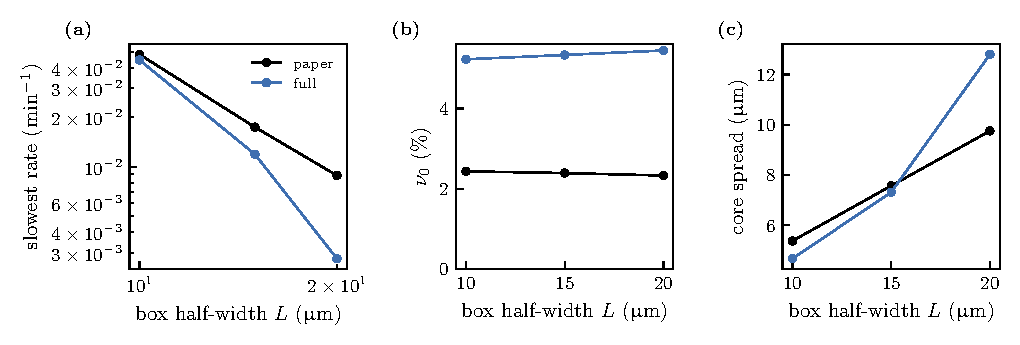
\includegraphics[width=\linewidth]{figures/fluct_box.pdf}
  \caption{Dependence on the box half-width $L$ at the fixed grid spacing $\Delta x=\nfhBox~\micron$: (a) the slowest
    relaxation rate, whose mode is a rigid translation of the defect; (b) $\nu_0$; (c) the
    standard deviation of the core position, $|(\sigma_x,\sigma_y)|$, from $\delta\Q$ at the core.}
  \label{fig:fluct-box}
\end{figure}

Near the core the order fluctuations are dominated by the motion of the defect. The two
slowest modes of the drift relax at $\nfslowPaper$ and $\nfslowBPaper~\minute^{-1}$ in the
paper's model ($\nfslowFull$ and $\nfslowBFull$ in the full model), and their $\delta\Q$ parts
overlap with the rigid translations $\partial_x\Q_\mathrm{ss}$ and $\partial_y\Q_\mathrm{ss}$ to at least
$\nftransFull$. Nothing but the wall restores a displaced defect, so these rates fall with the box
(\cref{fig:fluct-box}a): from $L=10$ to $20~\micron$ by a factor of $5.5$ in the paper's
model and $16$ in the full model, about as $L^{-2.5}$ and $L^{-4}$. Linearizing $q(\r)\simeq q(\mathbf 0)+\mathbf J\r$
about the core, the covariance of $\delta q(\mathbf 0)$ gives the spread of the core position,
which grows with the box to $\nfcorePaperTwenty$ and $\nfcoreFullTwenty~\micron$ at $L=20~\micron$. The defect therefore wanders over
distances comparable to the box, and only the wall keeps the linearization meaningful. The
density variance hardly cares: between $L=10$ and $20~\micron$, $\nu_0$ changes from
$\nfnuPaperTen$ to $\nfnuPaperTwenty\%$ in the paper's model and from $\nfnuFullTen$ to $\nfnuFullTwenty\%$ in the full model
(\cref{fig:fluct-box}b), because the density fluctuations are local, over $\ell_\mathrm n$, and
follow the noise much faster than the defect moves. A translation mode that is slow and only
weakly damped by the wall is also consistent with the earlier observation that the slowest rate of the paper's runs falls with the
box, and that coarse grids or large boxes make it positive.

\begin{figure}[t]
  \centering
  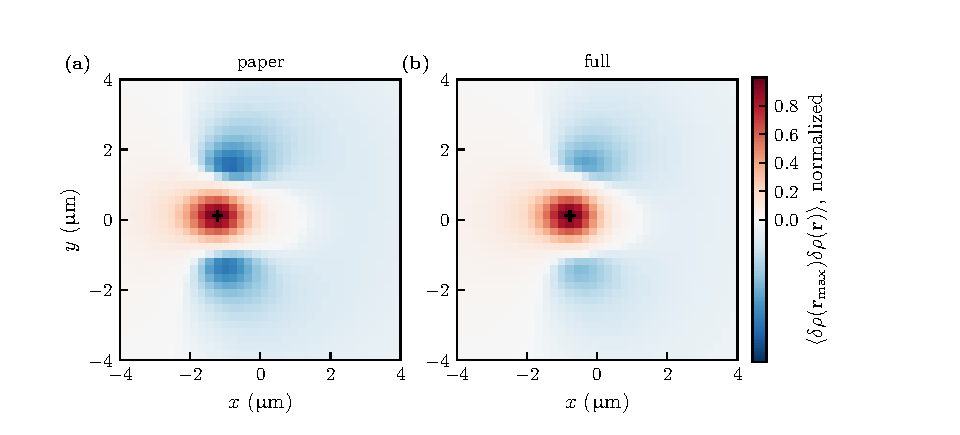
\includegraphics[width=0.9\linewidth]{figures/fluct_corr.pdf}
  \caption{Correlation coefficient of $\delta\rho(\mathbf r_\mathrm{max})$ with $\delta\rho(\r)$,
    paper (a) and full model (b).}
  \label{fig:fluct-corr}
\end{figure}

The density correlation around the point of maximum variance (\cref{fig:fluct-corr}) decays
over the cutoff length and has two weak anticorrelated lobes above and below the axis, in
both models. The full model leaves its shape unchanged.

\begin{updenv}
\subsection{A reduced model for the density variance}
\label{sec:fluct-reduced}
The splits above say which parts of the fluctuating equations the density variance needs,
and they suggest a simpler model that keeps only those parts. Its justification is the
separation of time scales. At the scale of the cutoff the density relaxes within
$\tau_c\approx0.4$~ms, while the order relaxes at most at $20~\minute^{-1}$, about $10^4$
times more slowly. Seen from the density, $\delta\Q$ is therefore frozen, and the equal-time
variance consists of the variance at fixed order, which is the direct pathway, and of the
density that follows the slow order, which the elastic and active forces suppress by
$\zeta/B$. We therefore drop the dynamics of $\delta\Q$ and, with it, every noise that acts
on $\Q$: the alignment flux $\bm\eta^{\Q}$, the rotational noise $\mathbf f^{\Q}$ and the
cross covariance of $\bm\eta_\rho$ and $\bm\eta^{\Q}$. We keep the whole covariance of
$\bm\eta_\rho$, the isotropic part and the part with $\Q_\mathrm{ss}$, the leading order in
$\rho-1$ and the same cutoff. The density then obeys
$\partial_t\delta\rho=(B/\xi_0)\nabla^2\delta\rho-\nabla\!\cdot\!\bm\eta_\rho$, and its
variance is the paper's eq.~total-gauss evaluated on the steady state of the full model.

The numbers support this. The order adds $\nfpathQFull\times10^{-4}$ of the pedestal through
its own variance and $\nfpathIFull\times10^{-4}$ through the interference term, so the net
correction is below $10^{-3}$, against $\nu_0=\nfnuFull\%$. In the enhancement of
eq.~R-value it changes $R$ by a factor of about $1.2$, which is small compared with the width
of the measured bin. The analytic formula on the full steady state gives $\nu_0=\nfnuAnFull\%$,
and the Lyapunov solution gives $\nfnuFull\%$. In the paper's model the lattice value,
$\nfnuPaper\%$, still rises with refinement toward the formula's $\nfnuAnPaper\%$.

The split also shows which simplifications are not consistent. The reversal noise is one
flux that carries both density and alignment, so its pieces cannot be dropped one at a time
while $\delta\Q$ remains dynamical. In the far field of the full model they shift the
variance by $\nfisoFarFull\%$, $\nfcrossFarFull\%$ and $\nfQQrevFarFull\%$ and cancel in the
sum, so dropping one of them makes an error as large as $\nu_0$ and can make the noise
covariance indefinite. The change of $\nu_0$ comes entirely from the steady state, so the
mean field has to be the full model even when the fluctuations are reduced, and its closure
has to be applied in all three places, because the exact moments of
\cref{eq:exact-moments} come from one distribution. The rung with the self-propulsion term
alone comes close to the full result only because the rotational friction and \upd{the $\nabla\H$
terms} shift $\nu_0$ in opposite directions. Finally, the paper's drift cannot be linearized
about the full steady state, which does not solve the paper's equations; the reduced model
avoids this, because it does not use the drift of $\Q$ at all.

The reduced model covers the equal-time density variance and the density correlations. It
says nothing about the order itself, whose director spread of about $30^\circ$ and wandering
core already strain the linear theory of $\delta\Q$.
\end{updenv}

% ======================================================================
\section{Open points}
\label{sec:open}

\begin{itemize}
  \item \emph{Larger boxes.} At $L=30~\micron$ ($N_\mathrm{int}=180$, $\Delta x=0.33~\micron$) the
    full model's translation mode is unstable, while the paper's is stable; the density variance
    is nearly the same as in the smaller boxes ($\nu_0=2.2\%$ and $5.0\%$). A finer grid in the
    large box would cost about four times the production run.
  \item {\color{OliveGreen}\emph{Reduced fluctuation model.} The density variance follows from
    eq.~total-gauss on the full steady state (\cref{sec:fluct-reduced}); the Lyapunov solve is
    needed only for the order fluctuations.}
  \item \emph{Linear order fluctuations.} The director fluctuates by about $30^\circ$ and the core
    position by several $\micron$, so the Gaussian theory of $\delta\Q$ is at the edge of its
    validity, and the core spread is set by the wall. The density variance, which is local, is
    not affected.
  \item \emph{Enhancement.} The full model's $\nu_0$ with the paper's $z_\infty$ overshoots the
    measured enhancement by two orders of magnitude; whether a refit of $B$ (or of $a$, $K$,
    see the next point) restores agreement is open.
  \item \emph{Parameters.} We kept the bare parameters, so the far-field order dropped from
    $0.90$ to $\numSInfUniform$ and the core changed with it. Comparing the two models at
    the same observed $S_0$ and core size would mean retuning $a$ and $K$ for the full model.
  \item \emph{Marginal mobility.} Even with the exact moments, the amplitude mobility
    $1-2S^2+g_2S^2$ is small in the ordered region ($0.10$ at $S=0.846$, $0.04$ at
    $S=0.9$), so the full model is stiff where the order is strong. A first continuation that
    switched on \upd{the $\nabla\H$ terms} directly from the paper's model, where $S_\infty=0.9$,
    did not converge even at $w_H=0.05$. All paths used here switch on $w_R$, which lowers $S$,
    before or together with \upd{the $\nabla\H$ terms}.
  \item \emph{Passive defect on the finest grid.} At $\zeta=0$ and refinement~2 Newton did
    not converge, neither from the Pad\'e seed nor from the interpolated refinement-1
    solution, while the active problem converges on the same grid. Near the core, where $S$ is
    small, the elastic flux contributes the anti-diffusion $(|a|/\xi_0)\nabla^2\Q=4.1\nabla^2\Q$,
    which at $\zeta=0$ exceeds the elastic relaxation $(4K/\xir)\nabla^2\Q=2.5\nabla^2\Q$; at
    $\zeta=12.5$ the self-propulsion term adds $(\zeta/\xi_0)\nabla^2\Q=2.5\nabla^2\Q$ to the
    latter. Whether this is the cause we did not check.
  \item \emph{Finite $B$.} The terms of relative order $\zeta/B$ are still dropped, as in the
    paper.
\end{itemize}

\end{document}
